\documentclass[12pt]{report}

\usepackage[a4paper, total={17cm, 25cm}]{geometry}
\usepackage{hyperref}
\usepackage{graphicx}
\usepackage{float}

\begin{document}

\title{Cooking Time}
\author{Nicola Camillucci \& Alessandro Passoni}

\begin{center}
\Large
\textbf{POLITECNICO DI MILANO}
\end{center}
\begin{figure}[H]
	\centering
	
\includegraphics{polimi}
\end{figure}
\vspace{1cm}

\begin{center}
\large
Design and Implementation of Mobile Applications\\
Prof. Luciano Baresi\\
2020/2021\\
\vspace{2cm}

\Huge
\textbf{COOKING TIME}\\
\vspace{5cm}

\Large
\textbf{Team Members:}\\
\begin{table} [H]
    \centering
    \large
    \begin{tabular}{||c | c | c||}
    \hline
     \textbf{ID} & \textbf{Surname} & \textbf{Name} \\
    \hline
    \hline
    944569 & Camillucci & Nicola \\
    \hline
    945105 & Passoni & Alessandro \\
    \hline
    \end{tabular}
\end{table}
\end{center}

\tableofcontents{}
\newpage

\thispagestyle{empty}
\newpage

\chapter{Introduction}

	\section{Purpose}
		The application has an academic purpose and in particular it is the project to grade the \textit{Design and Implementation of Mobile Application} master level degree course taught by professor Luciano Baresi at Politecnico di Milano.
		The project assignment asks to design and implement a mobile application using one of the four technologies presented during the lectures, the platform can be chosen by the students. 

		This document illustrates all the design and implementation decision related to CookingTime app made by Nicola Camillucci and Alessandro Passoni. 
		It provides as well a guidance to implement all the features of the app according to the decided design, and also to present the project to people not involved into the development process.


	\section{Scope}
		The aim of this application is to allow people to share their own homemade recipes and to search for new ones among the variety of recipes posted by other people, in this way users will be able to share their tradition but also to find new way to cook any kind of dishes.
		Selecting a new recipe will be helped by ratings and reviews of people who have already cooked that recipes and if they want, they can also save it in a personal digital recipe book section.
		These are obtained thank to a database which can filter and suggest the right recipes to accomplish the request of the users.


	\section{Stakeholders}
		The main stakeholder of the project are professor Luciano Baresi and his teaching assistant Giovanni Quattrocchi that are going to evaluate the application.
		Moreover users interested in this application can be considered stakeholders as well.


	\section{Time Constraints}
		There were no defined deadlines, except for the final delivery of the project on one of the exam date of the academic year.
		However the developers decided to split the work into three milestone deadlines which are on a generic and flexible date. 
		The aim is to have a sort of check points, usually named as alpha, beta and final version, in order to have some deliverable part incrementally.
		This will help to not encounter some issues about parts developed at the beginning of the implementation during the further steps of the development.
		The implementation started in the second half of November 2020 and it's planned to end by the first half of February 2021.


	\section{Risk Analysis}
		In the first phase of the development process the team identified the possible risks related to the implementation of this type of application, in order to train ourselves how to deal and avoid all these kind of issues.
		The most critical feature to deal with is the interaction with the database and the authentication phase.


	\section{Overview}
		The document is structured as follows:
		TODO
		\begin{itemize}
			\item \textbf{Section 1: Introduction.} A general introduction of the Design Document. The objective is to explain what the document is going to address.

			\item \textbf {Section 2: General Overview.} A general overview of the project. In this section, the reader can find the main features of the application and
			the requirements of the application.

			\item \textbf{Section 3: Architectural Design.} This section contains an overview of the high-level components of the system and then a more detailed 
			description. Finally, it shows the Component Interfaces and the chosen architectural styles and patterns and also the database structure.
			
			\item \textbf{Section 4: User Interface Design.} This section contains the screenshots of the application with some descriptions of the user interfaces 
			and how to move through the application screens.
			
			\item \textbf{Section 5: Frameworks, External services and Libraries.} This section aims to explain the main frameworks, external services and libraries used 
			pointing out their advantages and possible disadvantages and why the team decided to use them.
			
			\item \textbf{Section 6: Test Case.} This section identifies how the application will be tested and shows a list test cases performed reporting their results.
			
			\item \textbf{Section 7: Effort and Cost Estimation.} A summary of worked time and cost estimation of the work.
			
			\item \textbf{Section 8: Future work.} This section presents some possible new feature which could be added further in time.
		\end{itemize}
\newpage
\chapter{General Overview}

\section{Concept}
	CookingTime is a multi-platform application that allows users to share their homemade cooking recipes with others and to search for new ones among the variety of recipes posted by other people.
	Furthermore users can save their favorite recipes in a personal recipe book in the app in order to always have them at hand and never lose them.
	Users will also be able to give suggestions by writing reviews and rate recipes of other users.
	To access these functionalities, user are required to register to the server via mail and password, Google account or Facebook account.
	The main components of the project are:
	\begin{itemize}
		\item The client side part, the application itself, which is the first point of interaction with the user.
		It allows the user to access all the functionalities of the app, the app will then automatically query the server-side database based on the user's requests.
		
		\item The server side part, fully made with the Firebase platform, contains the relational database used to store all the users data, which comprehend user's login information, recipes and reviews.
	\end{itemize}


\section{Core features}
	This section of the document is devoted to present the main functionalities provided by CookingTime, to let the reader understand better these features, 
	they are divided by screen in which they are implemented.
	
	\subsection{Authentication Screen}
		\begin{itemize}
			\item Allows the user to register his/her-self in the application.
		
			\item Allows the user to authenticate using his/her email and password.
			
			\item Allows the user to authenticate using his/her Facebook account.
			
			\item Allows the user to authenticate using his/her Google account.
		\end{itemize}

	\subsection{Home Screen}
		\begin{itemize}
			\item Allows the user to see the latest posted recipes from all the other users.
			
		\end{itemize}

	\subsection{Write a Recipe Screen}
		\begin{itemize}
			\item Allows the user to post a recipe.
			
			\item Allows the user to upload a picture representing the recipe.
			
			\item Allows the user to insert a description, category, difficulty and preparation time of the recipe.
			
			\item Allows the user to add up to 10 steps for the preparation process of the recipe, each one including title, description and a photo.
		\end{itemize}

	\subsection{Search for Recipes Screen}
		\begin{itemize}
			\item Allows the user to filter recipes depending on categories, difficulty, rating and preparation time.
		\end{itemize}

	\subsection{Write a Review Screen}
		\begin{itemize}
			\item Allows the user to insert a rating and a text review of a recipe.
		\end{itemize}

	\subsection{Saved Recipes List Screen}
		\begin{itemize}
			\item Allows the user to see all his/her saved recipes.
		\end{itemize}

	\subsection{Account Settings Screen}
		\begin{itemize}
			\item Allows the user modify his/her personal information.
			
			\item Allows the user to see all his/her posted recipes.
			
			\item Allows the user to see his/her personal statistics.
			
			\item Allows the user to sign out from his/her account.
		\end{itemize}


\section{Functional Requirements}
	In this section we present the functional requirements necessary to the correct behavior of the system.

	\subsection{General Requirements}
		\begin{itemize}
			\item The application should be comprehensible by as many people as possible, so we decided to use the English language.
		\end{itemize}

	\subsection{Authentication Requirements}
		\begin{itemize}
			\item The \textit{Login screen} should be accessible only to users not currently logged in.
			\item The \textit{Login screen} should allow the user to login using email and password, or Facebook, or Google.
			\item The \textit{Register screen} should allow users to register using email, password and providing a username. 
			\item \textit{Authentication screens} should redirect the user to the Home screen if the authentication is successful.
		\end{itemize}

	\subsection{Home Requirements}
		\begin{itemize}
			\item The \textit{Home screen} should provide access to the user to all the application functionalities.
			\item The \textit{Home screen} should show to the user the latest recipes published by all the users.
			\item The \textit{Home screen} should provide access to the \textit{Recipe screens} by pressing on a specific recipe.
		\end{itemize}

	\subsection{Recipe View Requirements}
	\begin{itemize}
		\item The \textit{Recipe screen} should all information about the requested recipe, which comprehend: title, subtitle, author, description, image, rating, difficulty, category, intolerance, servings, time required, ingredients, steps and users's reviews.
		\item The \textit{Recipe screen} should also provide the \textit{Write a Review widget}.
		\item The \textit{Recipe screen} should allow the user to save the recipe in his saved recipes list.
	\end{itemize}

	\subsection{Write a Recipe Requirements}
		\begin{itemize}
			\item The \textit{Write a Recipe screen} should allow the user to provide all the necessary information needed to publish a recipe.
			\item The \textit{Write a Recipe screen} should allow the user to add images from both the gallery and the camera.
			\item The \textit{Write a Recipe scree}n should tell the user if some information are missing.
			\item After a recipe has been submitted it should be shown at the top of the \textit{Home screen}.
		\end{itemize}

	\subsection{Search for Recipes Requirements}
		\begin{itemize}
			\item The \textit{Search a Recipe screen} should allow all user to filter the recipes in the database based on difficulty, category, preparation time and intolerance.
			\item The \textit{Search a Recipe screen} should allow all user to sort the recipes in the database based on rating or submission time.
		\end{itemize}

	\subsection{Review Requirements}
		\begin{itemize}
			\item The \textit{Reviews widget} should allow the user to read the most recent reviews about the current recipe in the screen.
			\item The \textit{Write a Review widget} should allow the user to rate and write a review about the current recipe in the screen.
			\item The \textit{Write a Review widget} should forbid the user to write a second review for the same recipe.
			\item The \textit{Write a Review widget} should forbid the author of the recipe to write a review for that recipe.
		\end{itemize}

	\subsection{Saved Recipes List Requirements}
		\begin{itemize}
			\item The \textit{Saved Recipes screen} should allow the user to access all the recipes previously saved.
			\item The \textit{Saved Recipes screen} should allow the user to remove some of the saved recipes.
		\end{itemize}

	\subsection{Account Settings Requirements}
		\begin{itemize}
			\item The \textit{Settings screen} should allow the user to change his username, profile image and password.
			\item The \textit{Setting screen} should allow the user to log out from his account.
			\item The \textit{Setting screen} should display the user's total recipes, reviews received, rating among his recipes and latest recipes written.
		\end{itemize}


\section{Non-Functional Requirements}
	These are the non-functional requirements that are necessary to guarantee a functional application:

\begin{itemize}
	\item \textbf{Portability}: Using a cross-platform implementation allows the application to run both in Android and iOS systems. The application could be run on different sized devices as well.
	
	\item \textbf{Usability}: All the features of the application are quite easy to be found as the design of the interfaces are very user-friendly in order to provide the best user experience.
	
	\item \textbf{Availability and Reliability}: The application must be always working and be connected to the Firebase platform.
	The downtime is strictly related to the one of Firebase, which is very low.
	In case of any kind of failure the application must be restored to a correct state as soon as possible.
	
	\item \textbf {Security}: As the user have different way to sign in the application and they are providing some personal data, the app must be implement some security actions. For this reason the connection between the application and the Firebase server are done using and encrypted communication through SHA-1 keys.
	
	\item \textbf{Extensibility}: The application is developed for some basic feature which can be increased over the time.
	
	\item \textbf{Maintainability}: The application was developed with a clear coding style by commenting all the part in order to let the code be readable to anyone who wants to touch it.
	
	\item \textbf{Nice User Interface}: It's important that user experience will be the best, for this reason the UI is very nice and simple.
\end{itemize}

\newpage
\chapter{Architectural Design}

\section{Overview}
	The application architecture is basically composed by three layers, two of which are provided by Google services as you can see in the following picture:

	TODO: picture

\section{Presentation Layer}
	The presentation layer is figured out by the mobile application which runs on a device. 
	It comunicate with the Application/Web Server to retrieve and send data according to the user will. 
	The communication are handled by some protected request to the Application Server. 
	The mobile application contains as well the most of the logic layer in order to render data coming from the server and in order to organize the data to be sent.

\section{Application/Web Server}

	TODO: Description

\section{Database Design}
	The database is the one provided by Firebase and it's a NoSQL database, so information are stored in a sort of semi-structured way.
	Using Google solution we can achieve \textbf{Durability and persistance of data} in order to have them alway available, 
	\textbf{Consistency} so the database is always in a consistent state, \textbf{Atomicity} in this way all the operation are completelly executed and 
	\textbf{Isolation} which means that every operation are executed isoleted and indipendetly from the other ones.
	
	\subsection{Database Structure}
	In order lo let the read understand better the structure, here is provided a translated E/R schema of the database implemented by the application.
	
	TODO: picture of simplified structure 

	\subsection{Database feature}
	The application database allows to:
	
	\begin{itemize}
		\item Login the application.
		\item Read stored data in order to retrieve what was post by other users.
		\item Data manipulation (CRUD operation) depending on user permissions over data.
	\end{itemize}
	
	
\section{Significative design decision}
\newpage
\chapter{User Interface Design}

\section{Navigation Overview}
In this section we are going to present the whole navigation structure of CookingTime application.
The starting decision was to make a simple structure of application screens in order to let users find all the required screen in few taps, as presented in the picture below.
\begin{figure}[H]
	\centering
	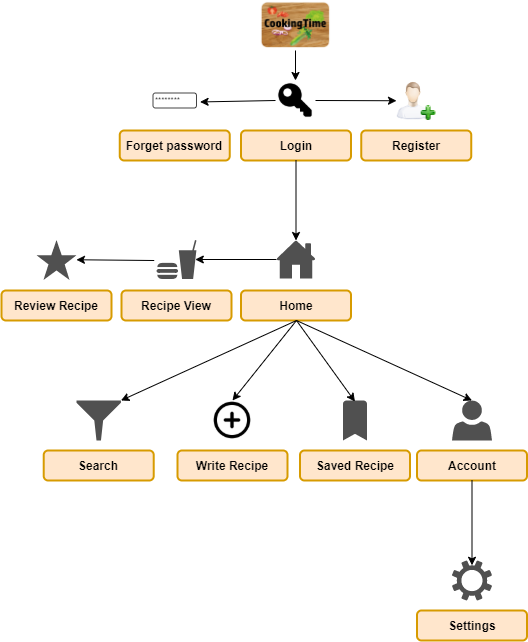
\includegraphics[width = .5\linewidth]{img/CookingTimeNavigator.png}
	\caption{App Navigation Structure}
\end{figure}

\section{Mockup screens}
In the following section there are some mockups of the application together with the explanation of all the feature reachable by the represented screen.

\subsection{Log In}
\begin{figure}[H]
	\centering
	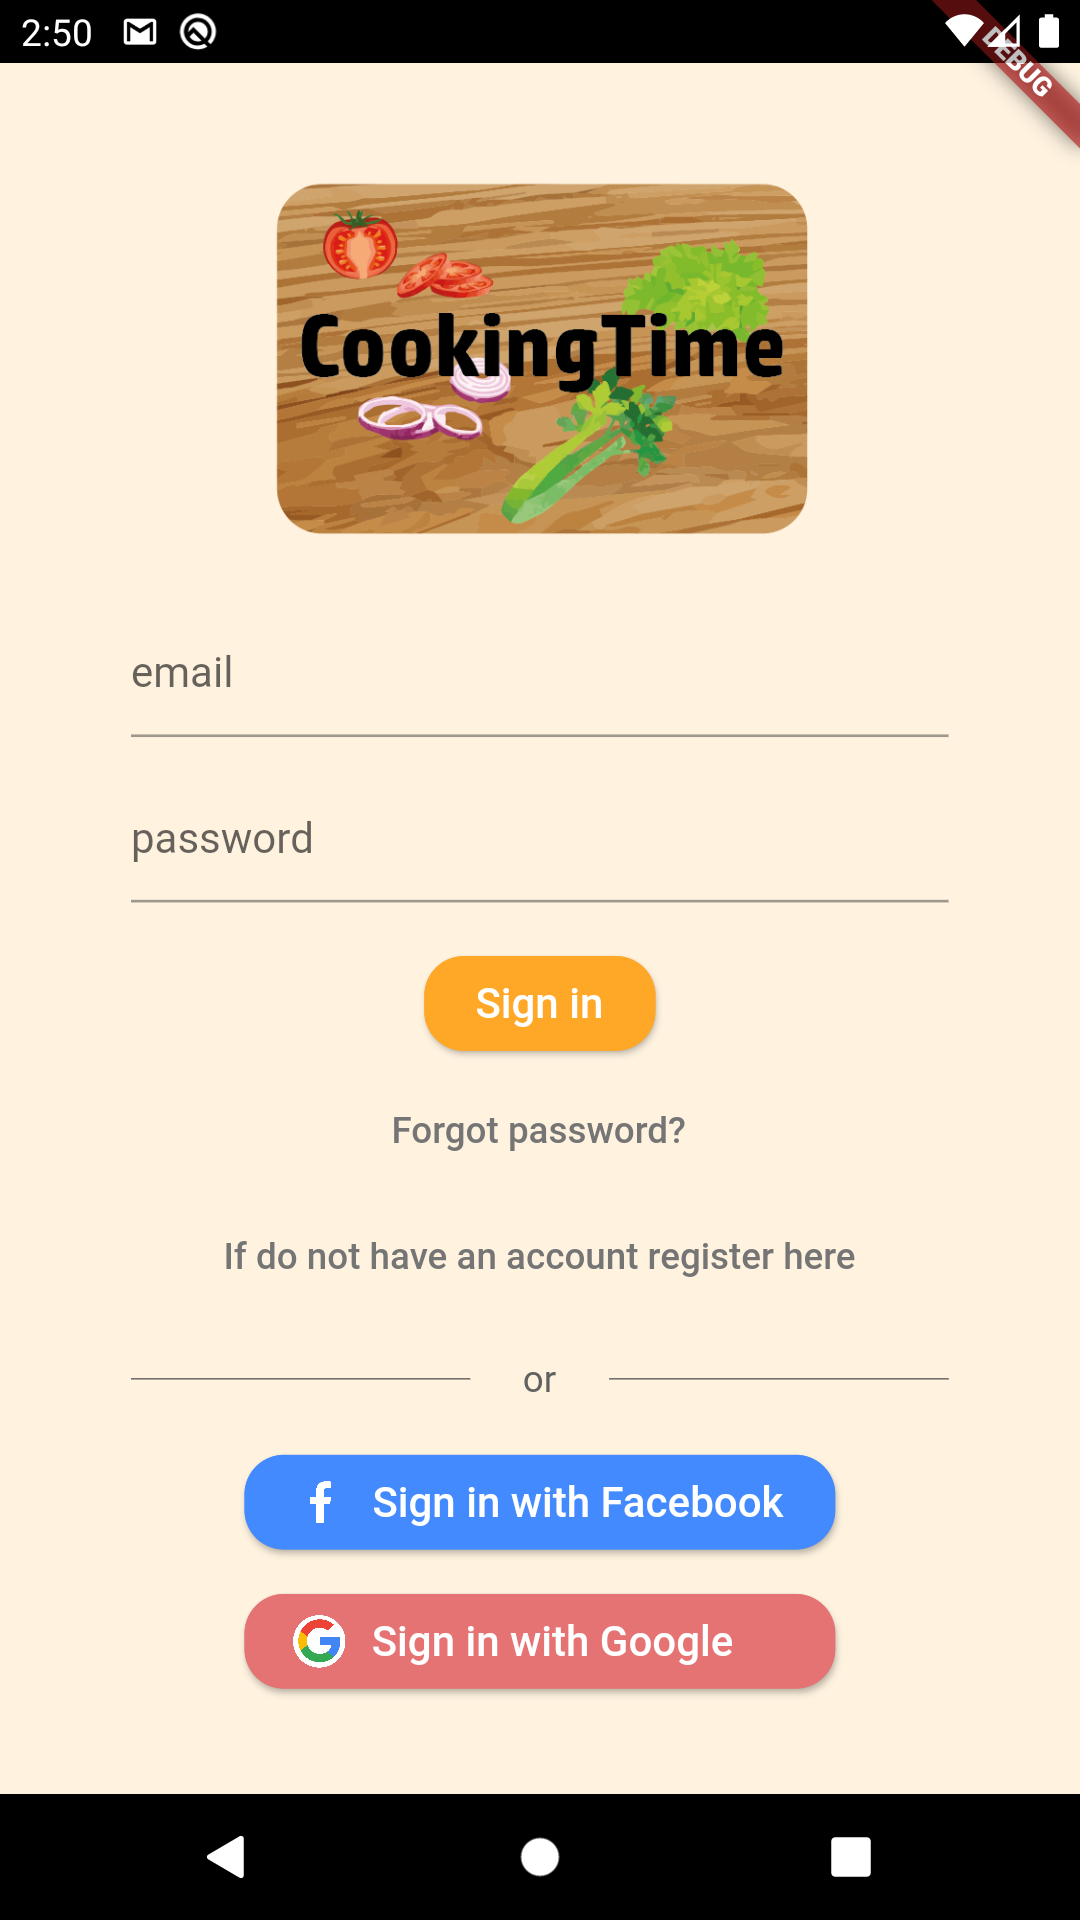
\includegraphics[width = .225\linewidth]{img/SignIn.png}
	\caption{Login Screen}
\end{figure}
This is the first screen which the user sees after the opening of the application, here he can login using his credentials, moreover he can go to the registration page or the lost password page.

\subsection{Registration}
\begin{figure}[H]
	\centering
	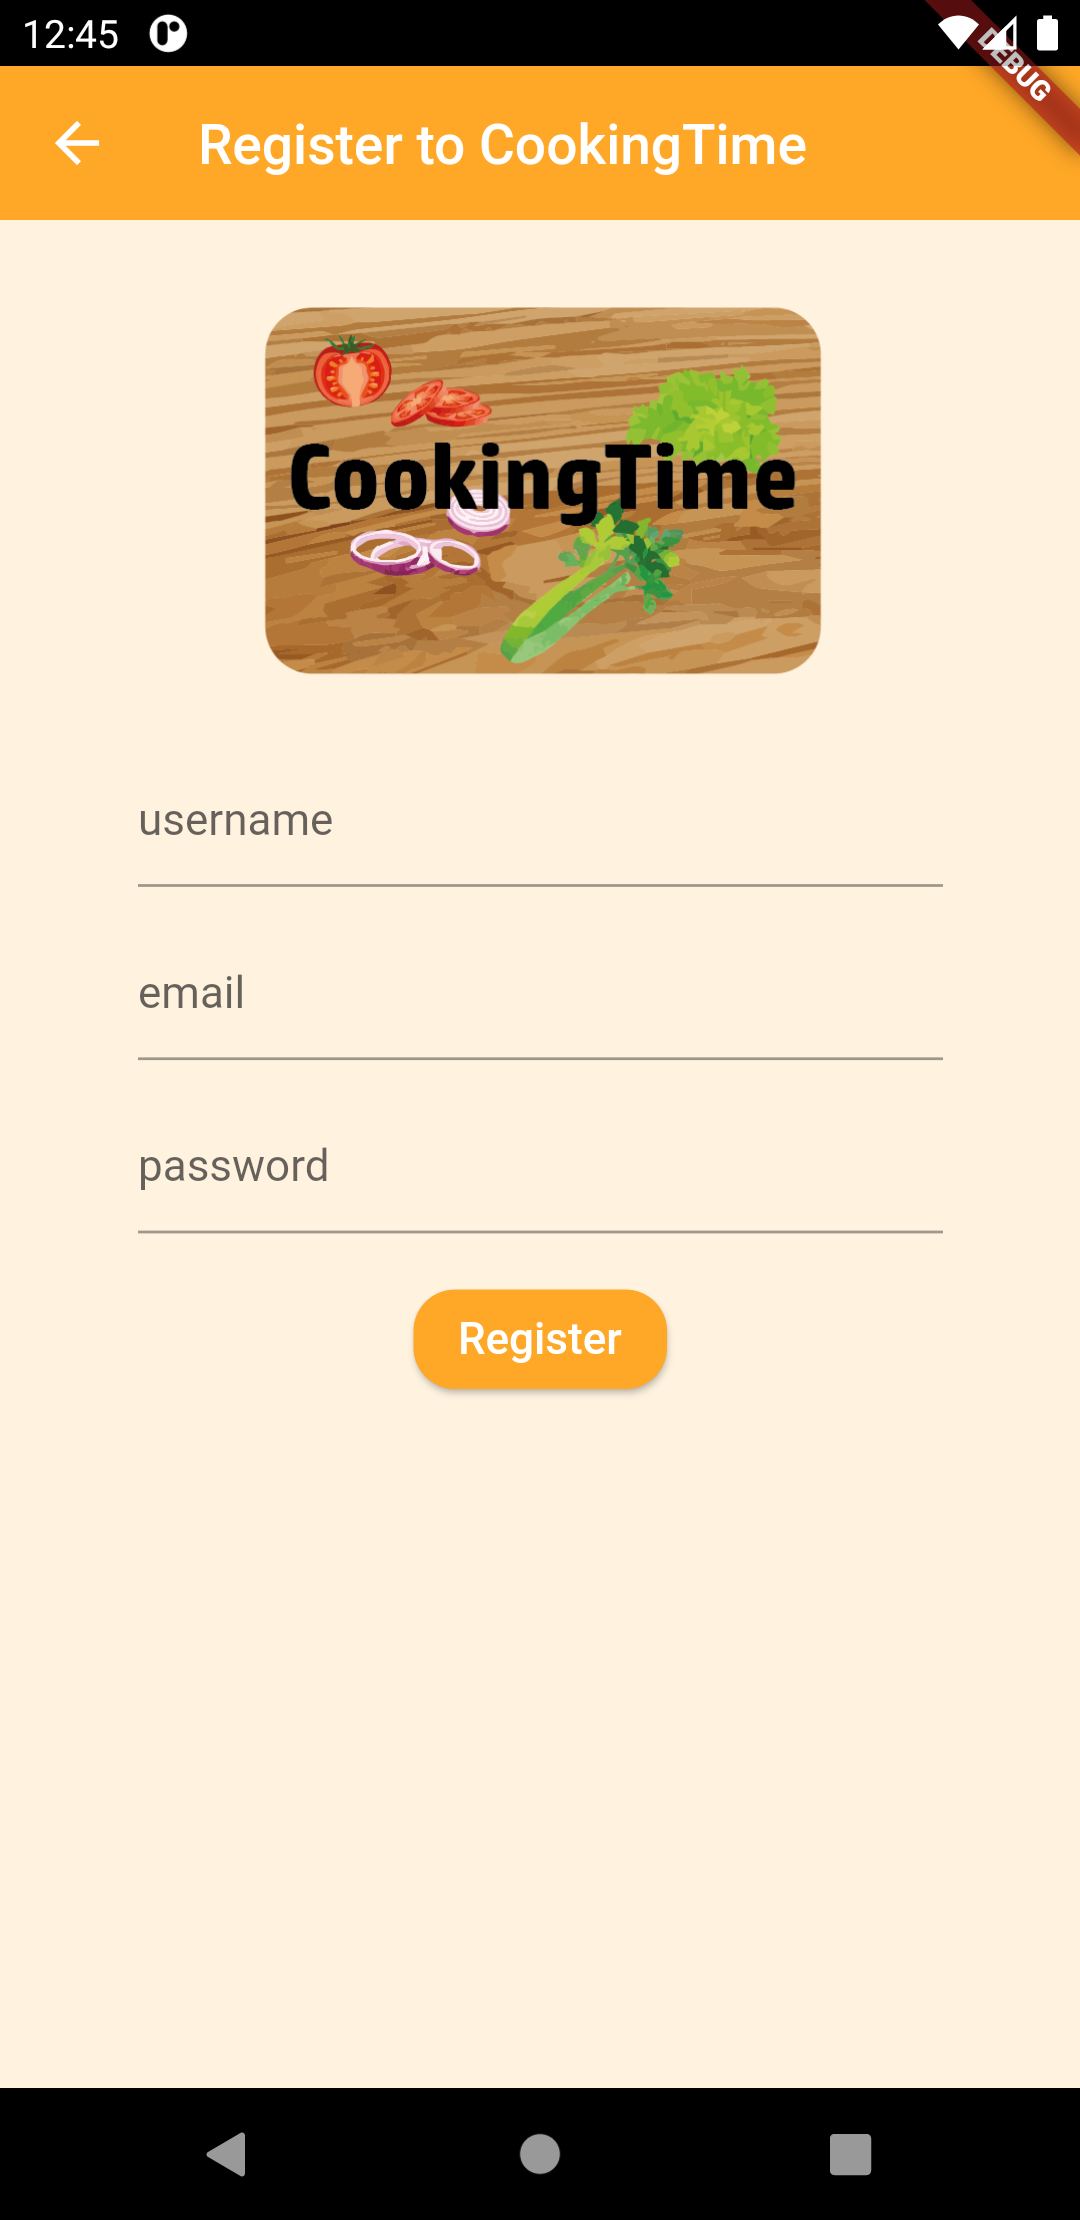
\includegraphics[width = .225\linewidth]{img/Registration.png}
	\caption{Registration Screen}
\end{figure}
This screen allows the user to register in the application providing a username, email and password.

\subsection{Password Reset}
\begin{figure}[H]
	\centering
	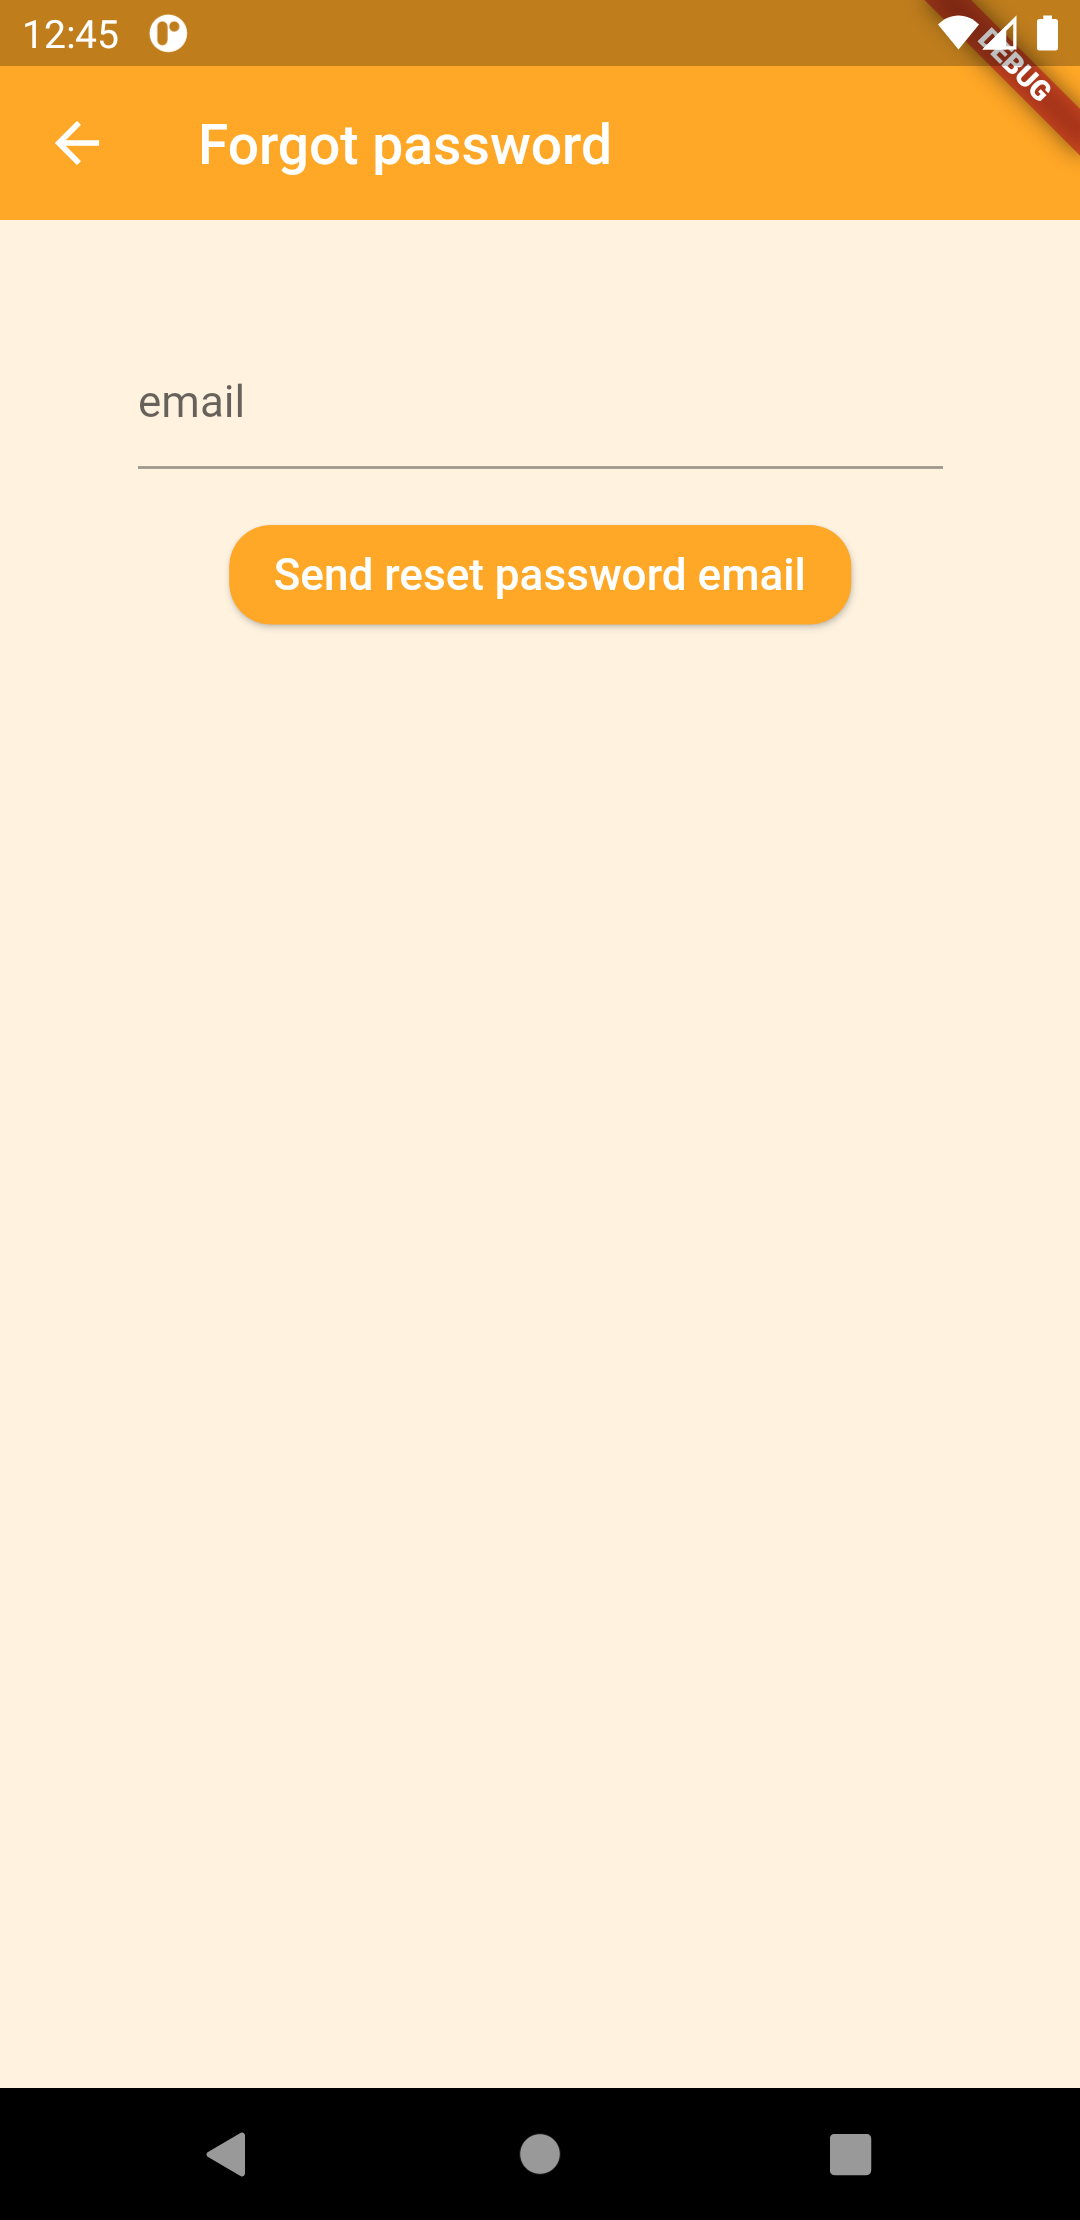
\includegraphics[width = .225\linewidth]{img/PasswordReset.png}
	\caption{Password Reset Screen}
\end{figure}
From this screen the user has the possibility to restore his lost password, providing the email by which he made the registration before.

\subsection{Home}
\begin{figure}[H]
	\centering
	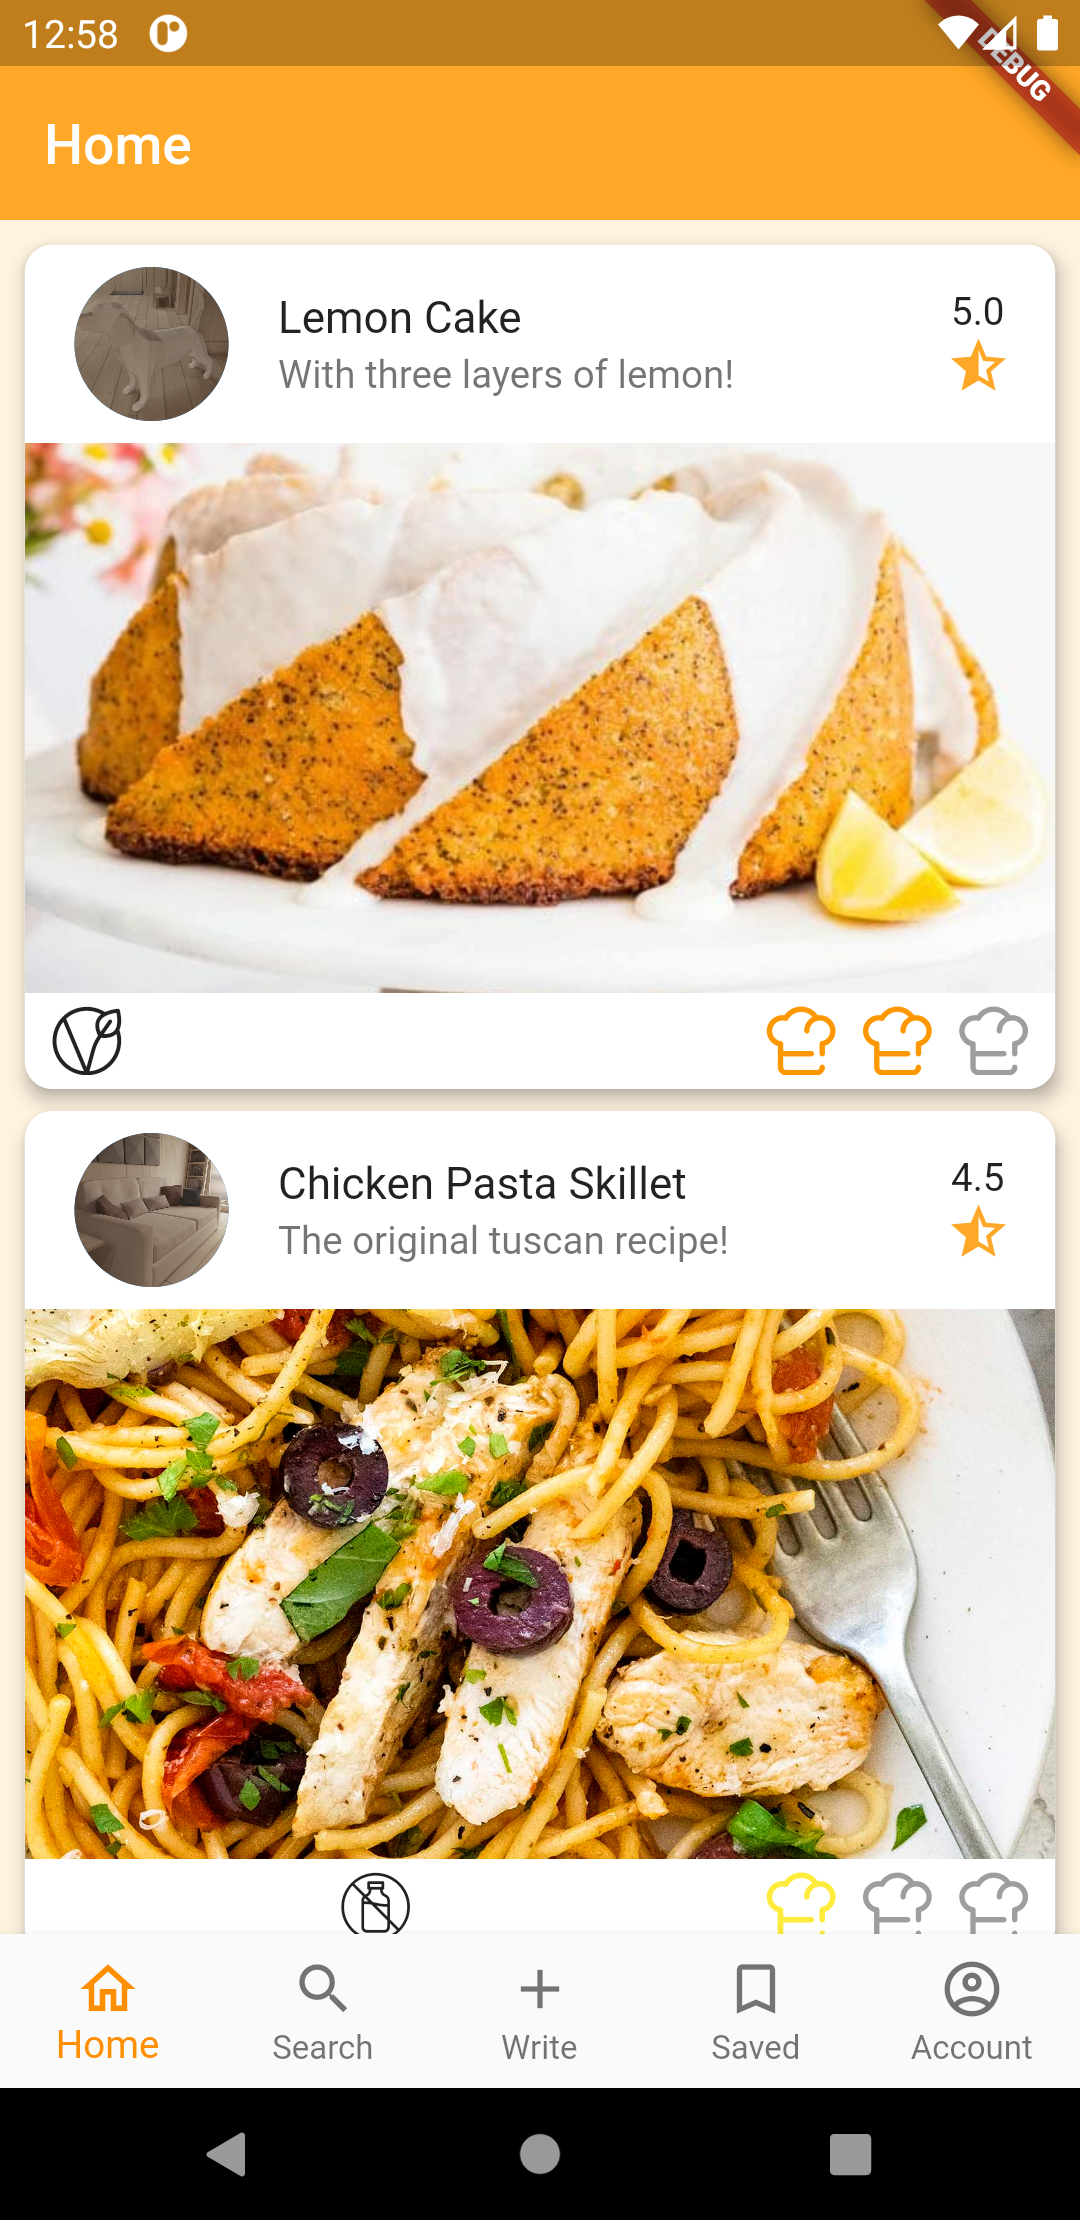
\includegraphics[width = .225\linewidth]{img/Home.png}
	\caption{Home Screen}
\end{figure}
This is the main screen of the application, from here the user is able to navigate to all the available screens and features of the application by using the navigation bar at the bottom.
It retrieves the ten most recent uploaded recipes and if he keeps scrolling more recipes are shown.

\subsection{Recipe Description}
\begin{figure}[H]
	\begin{minipage}{0.48\textwidth}
		\centering
		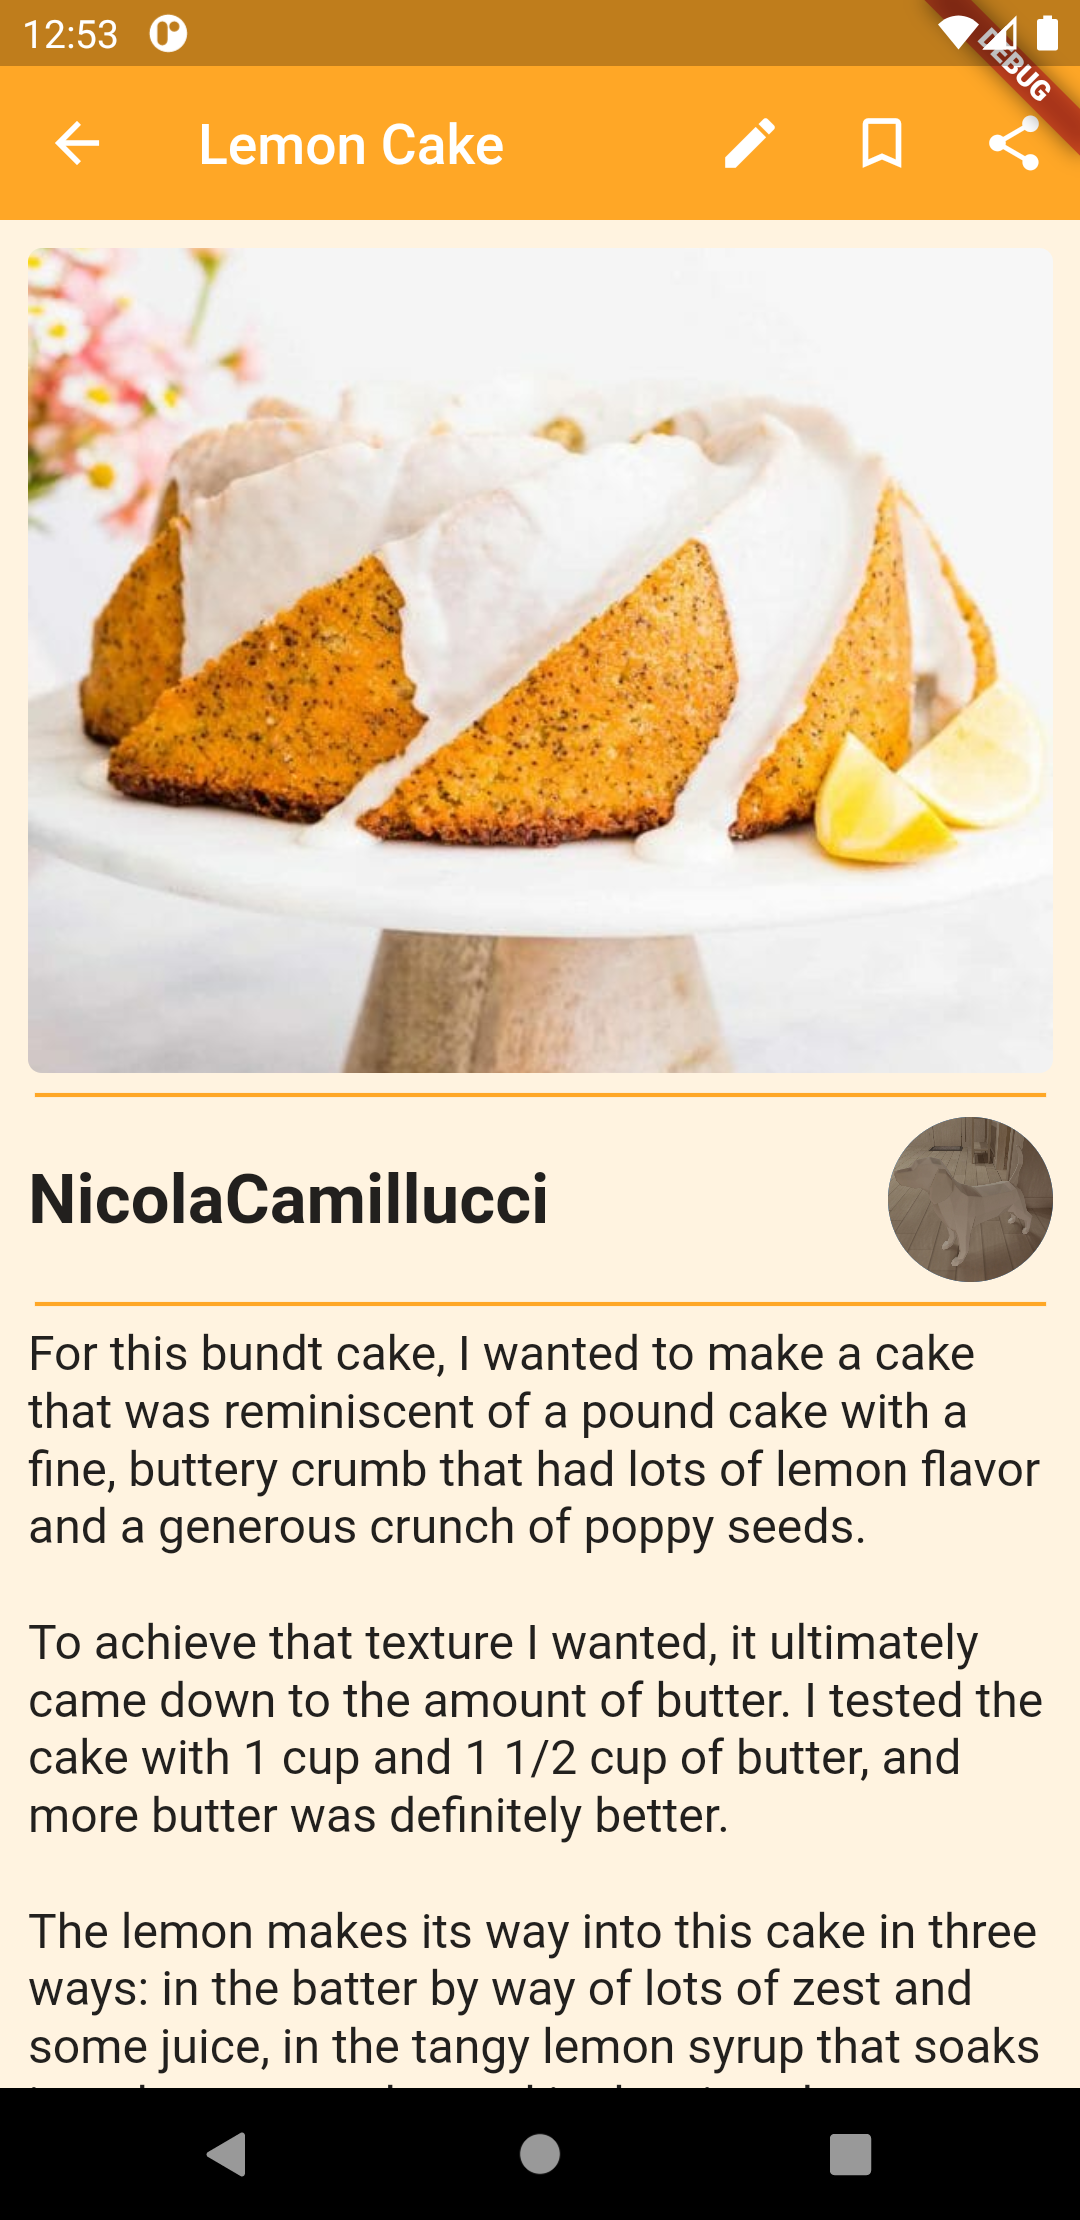
\includegraphics[width = .45\linewidth]{img/RecipeView.png}
		\caption{Recipe View 1 Screen}
	\end{minipage}\hfill
	\begin{minipage}{0.48\textwidth}
		\centering
		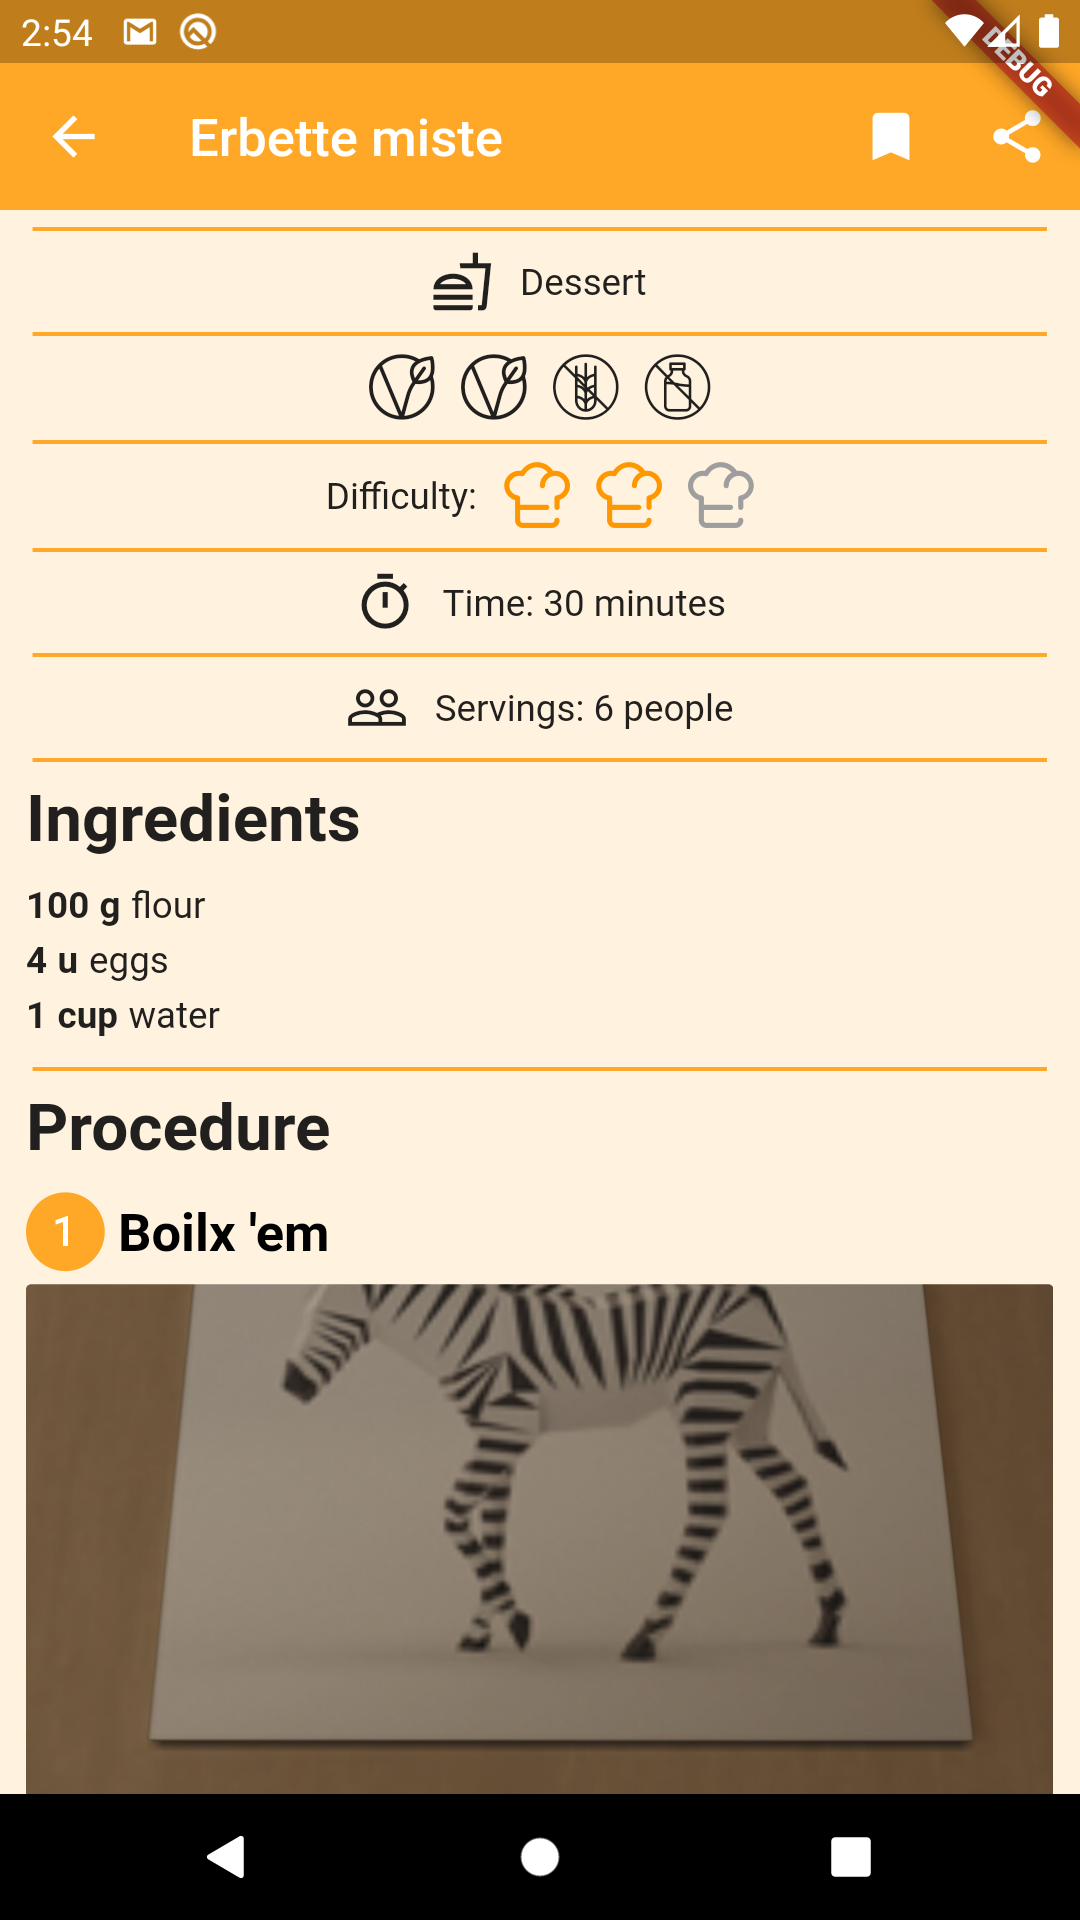
\includegraphics[width = .45\linewidth]{img/RecipeView_2.png}
		\caption{Recipe View 2 Screen}
	\end{minipage}
\end{figure}
This is the screen which appears after clicking on a recipe card.
In the first part it shows the picture of the dish, the author, category, intolerances, difficulty, average preparation time and suggested number of serving.
Then it shows the list of required ingredients and all the procedure to cook the recipe.
At the bottom of this view there is also the list of reviews left by other users, if any.

\subsection{Write a Recipe}
\begin{figure}[H]
	\begin{minipage}{0.31\textwidth}
		\centering
		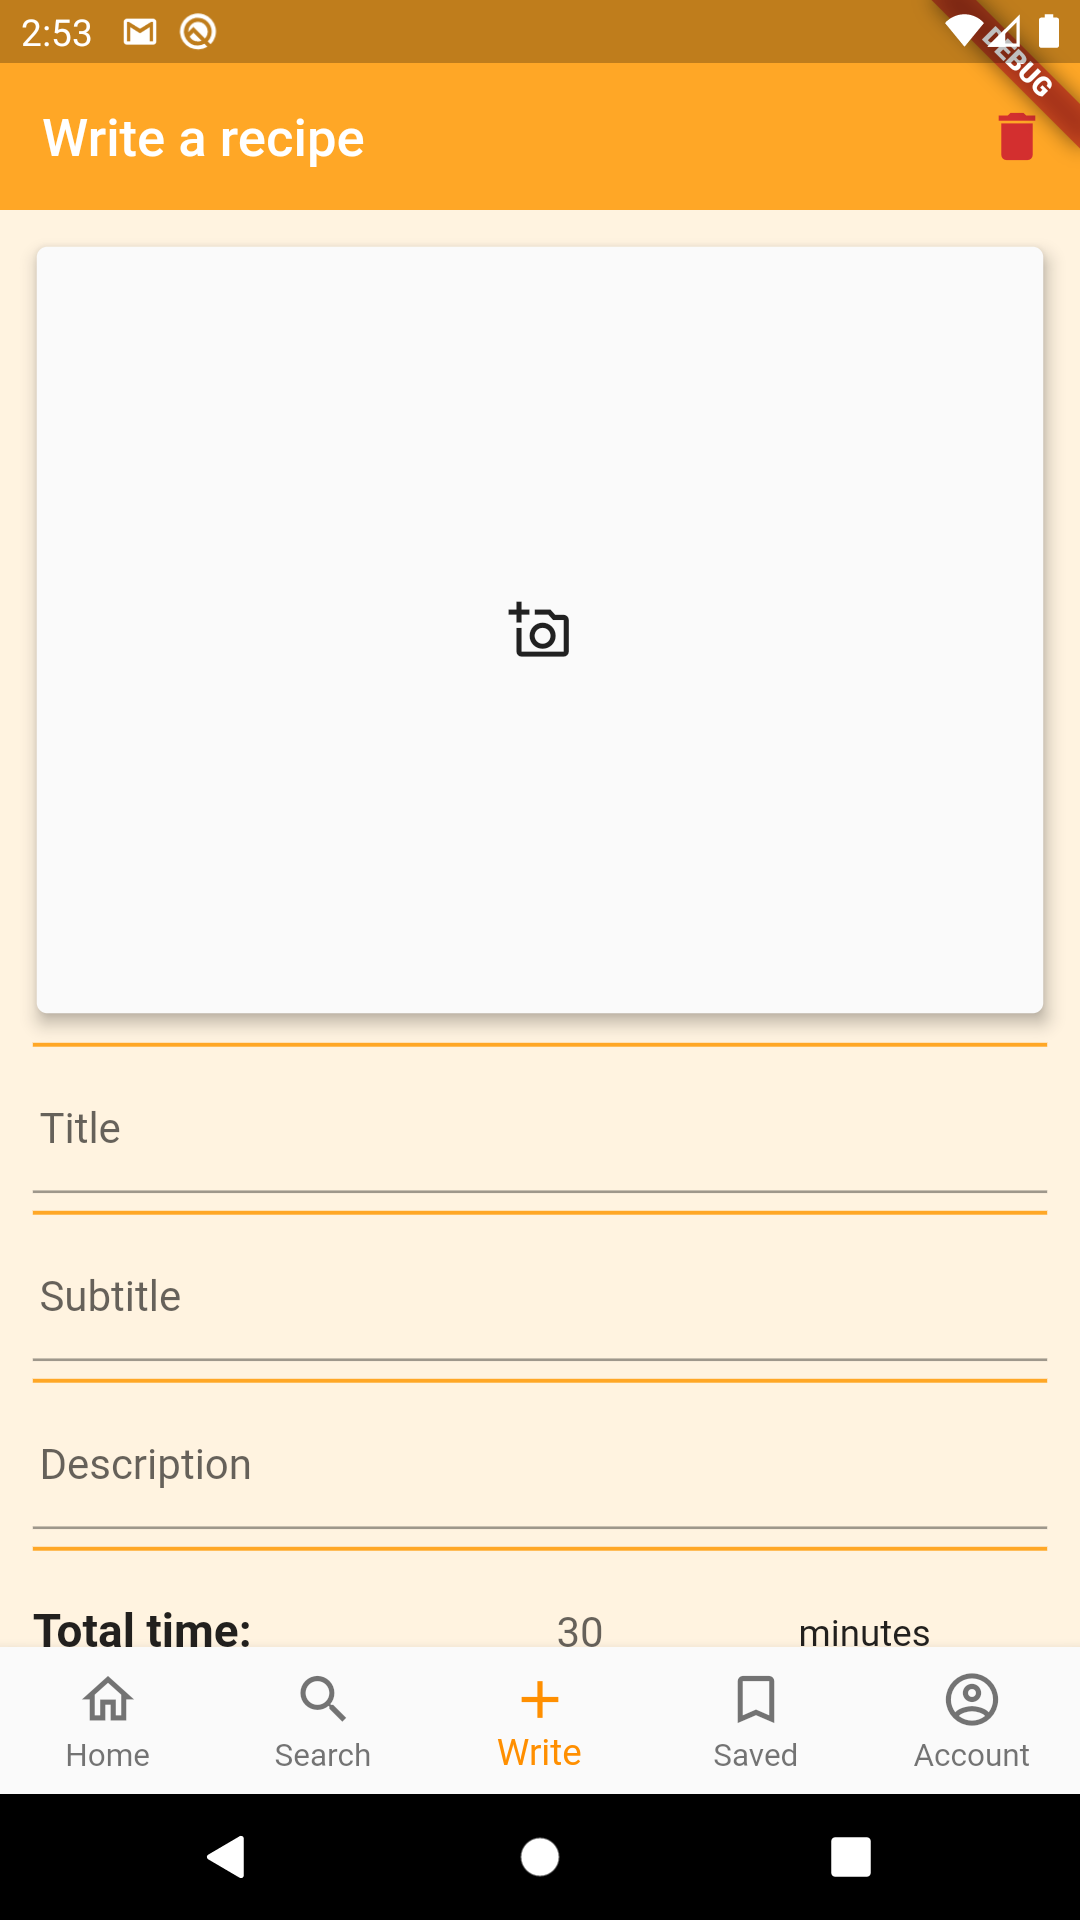
\includegraphics[width = .7\linewidth]{img/Write_1.png}
		\caption{Write Recipe 1 Screen}
	\end{minipage}\hfill
	\begin{minipage}{0.31\textwidth}
		\centering
		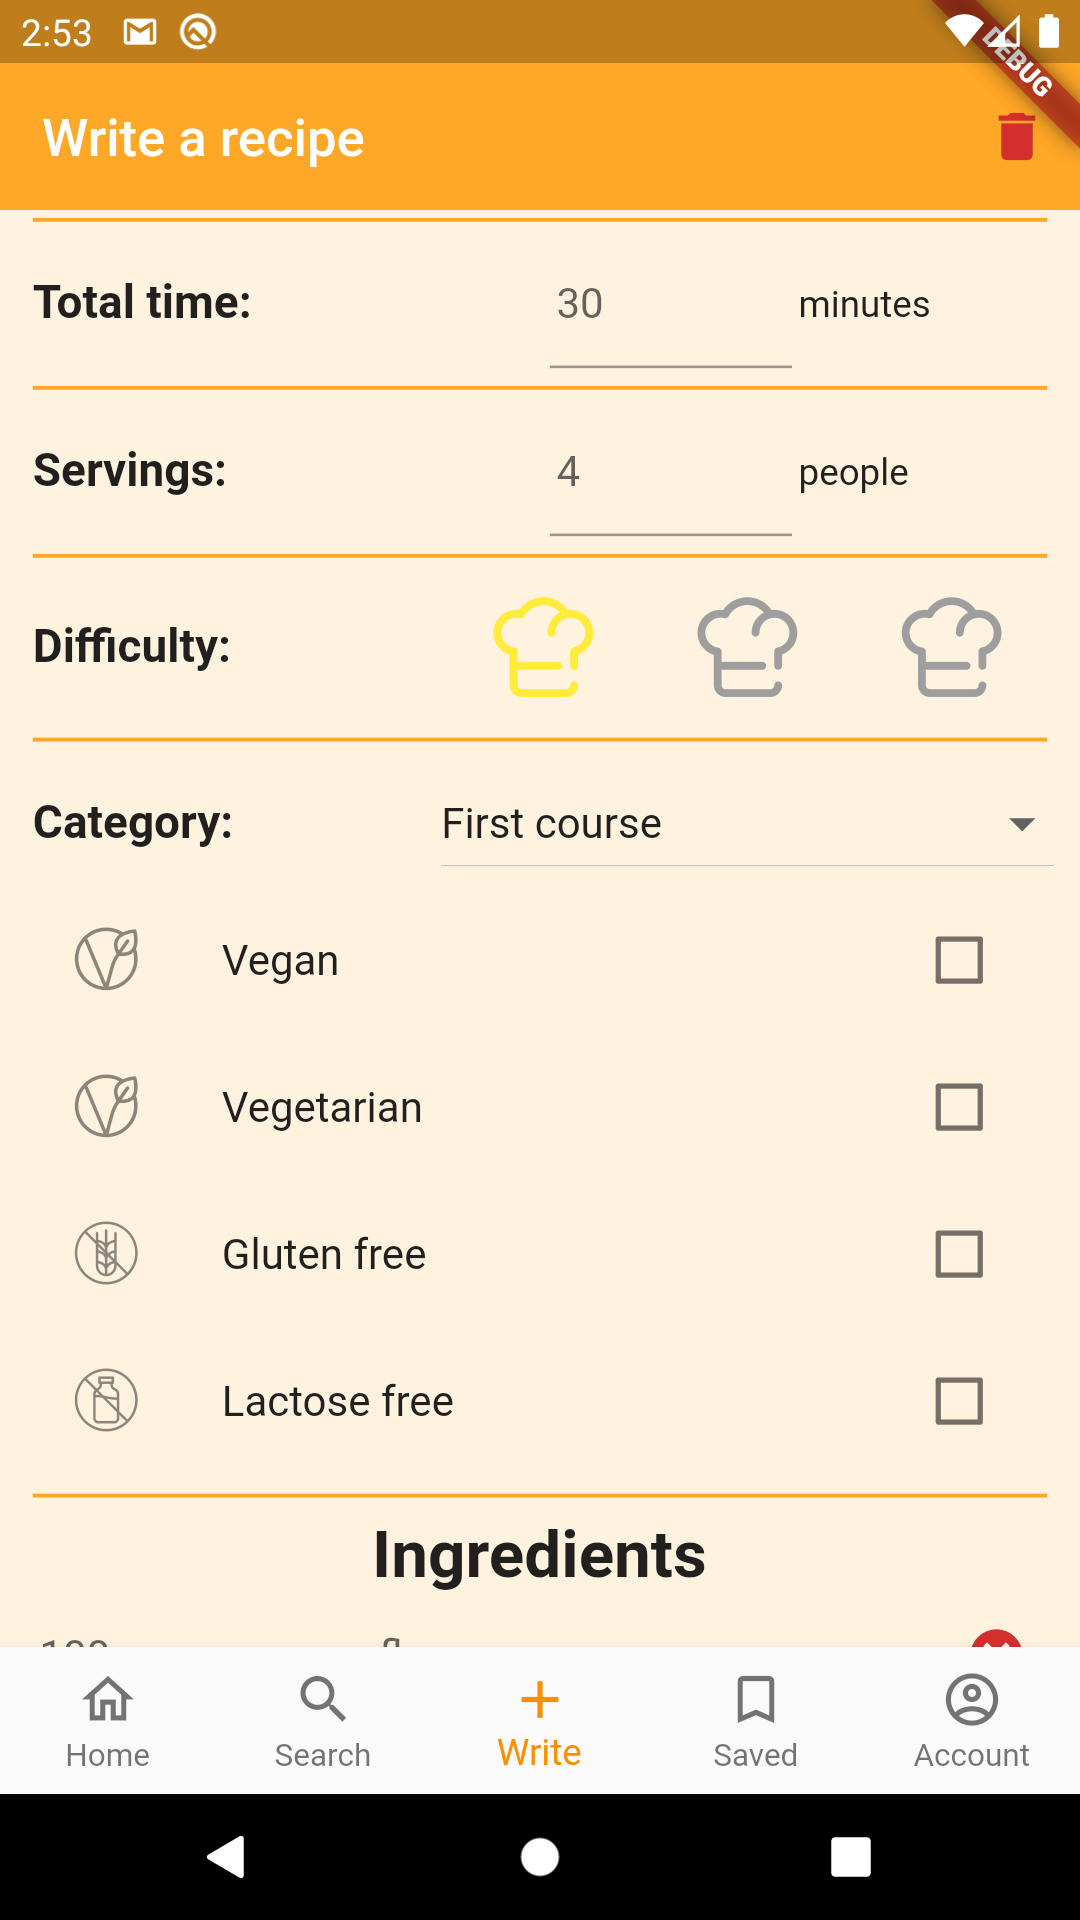
\includegraphics[width = .7\linewidth]{img/Write_2.png}
		\caption{Write Recipe 2 Screen}
	\end{minipage}\hfill
	\begin{minipage}{0.31\textwidth}
		\centering
		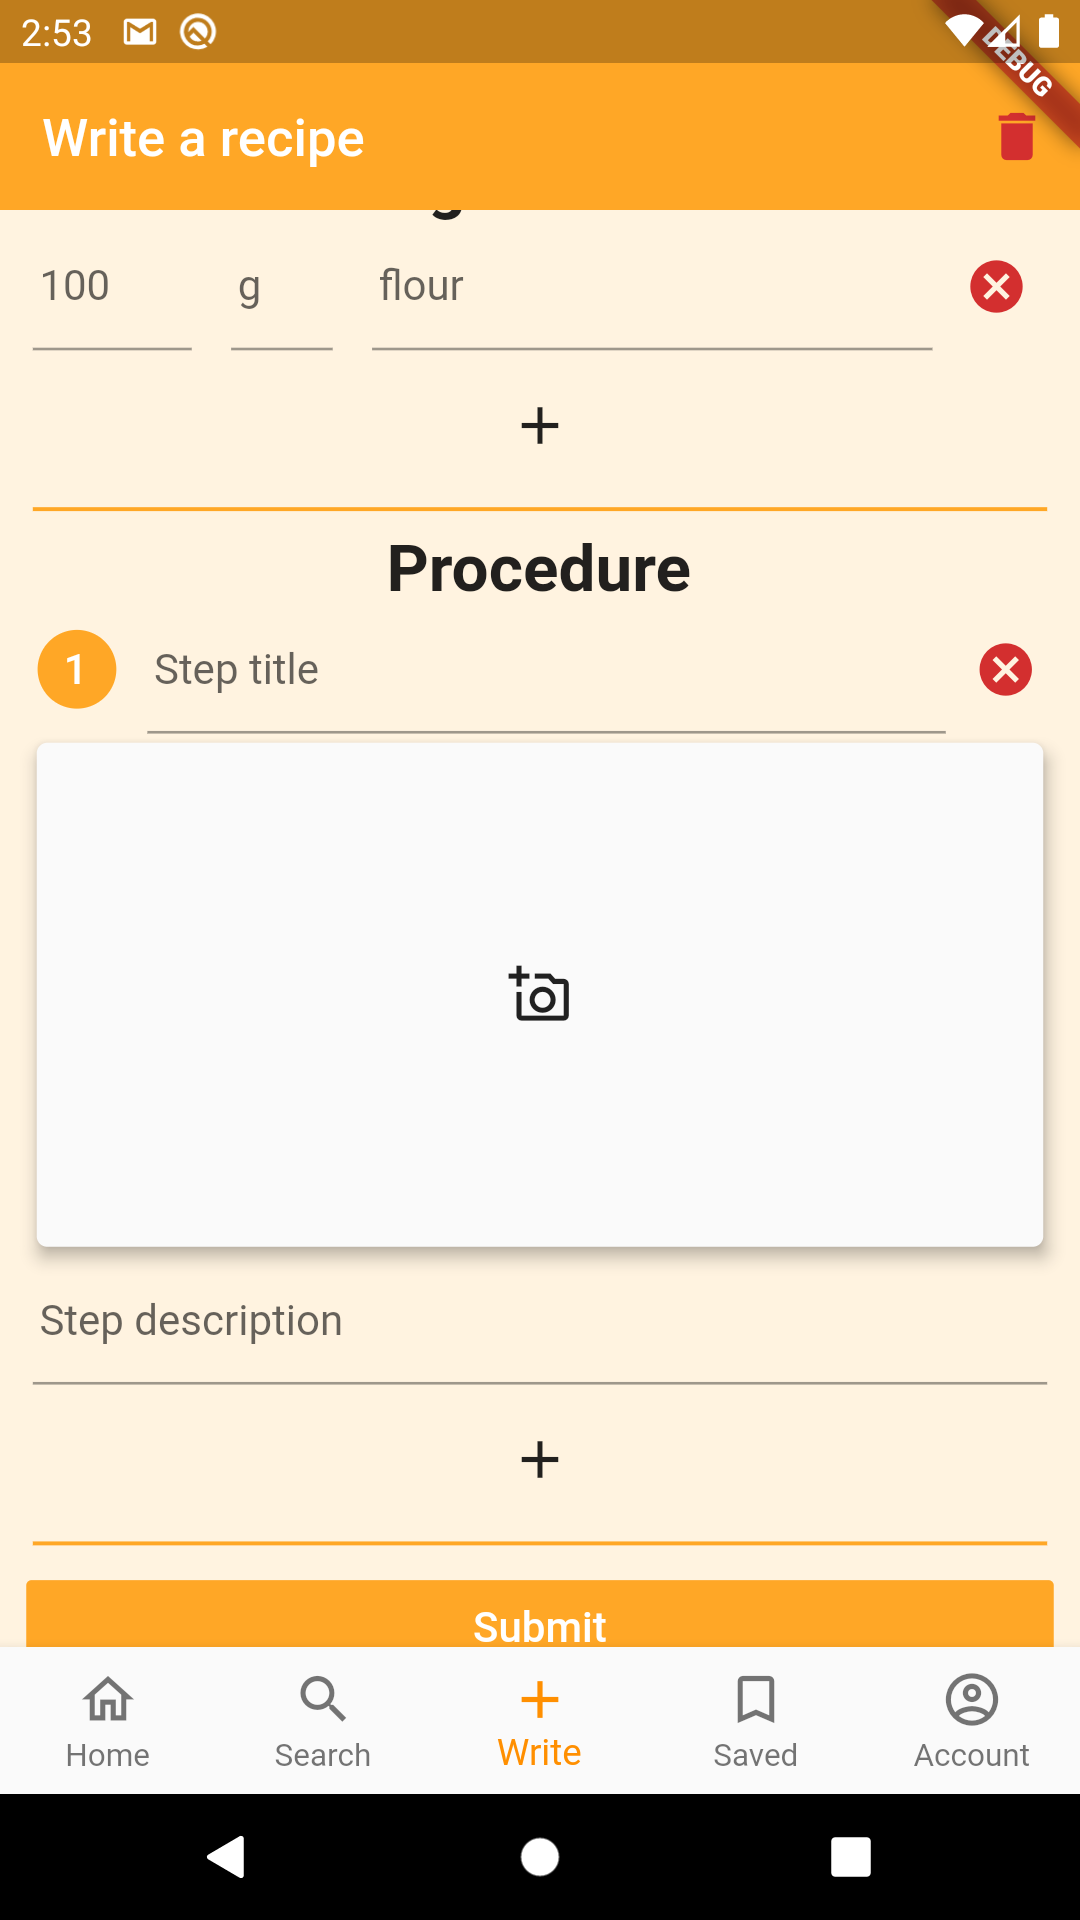
\includegraphics[width = .7\linewidth]{img/Write_3.png}
		\caption{Write Recipe 3 Screen}
	\end{minipage}
\end{figure}
This is the screen used in order to insert a new recipe, which it's reachable from the home page.
Here the user can provide the name of the recipe, the picture of the dish, some information like preparation time, suggested number of serving and intolerances, and especially the ingredients and procedure steps.
The submit button checks that all required information are inserted by the user before saving the recipe into the database.

\subsection{Search Recipes}
\begin{figure}[H]
	\centering
	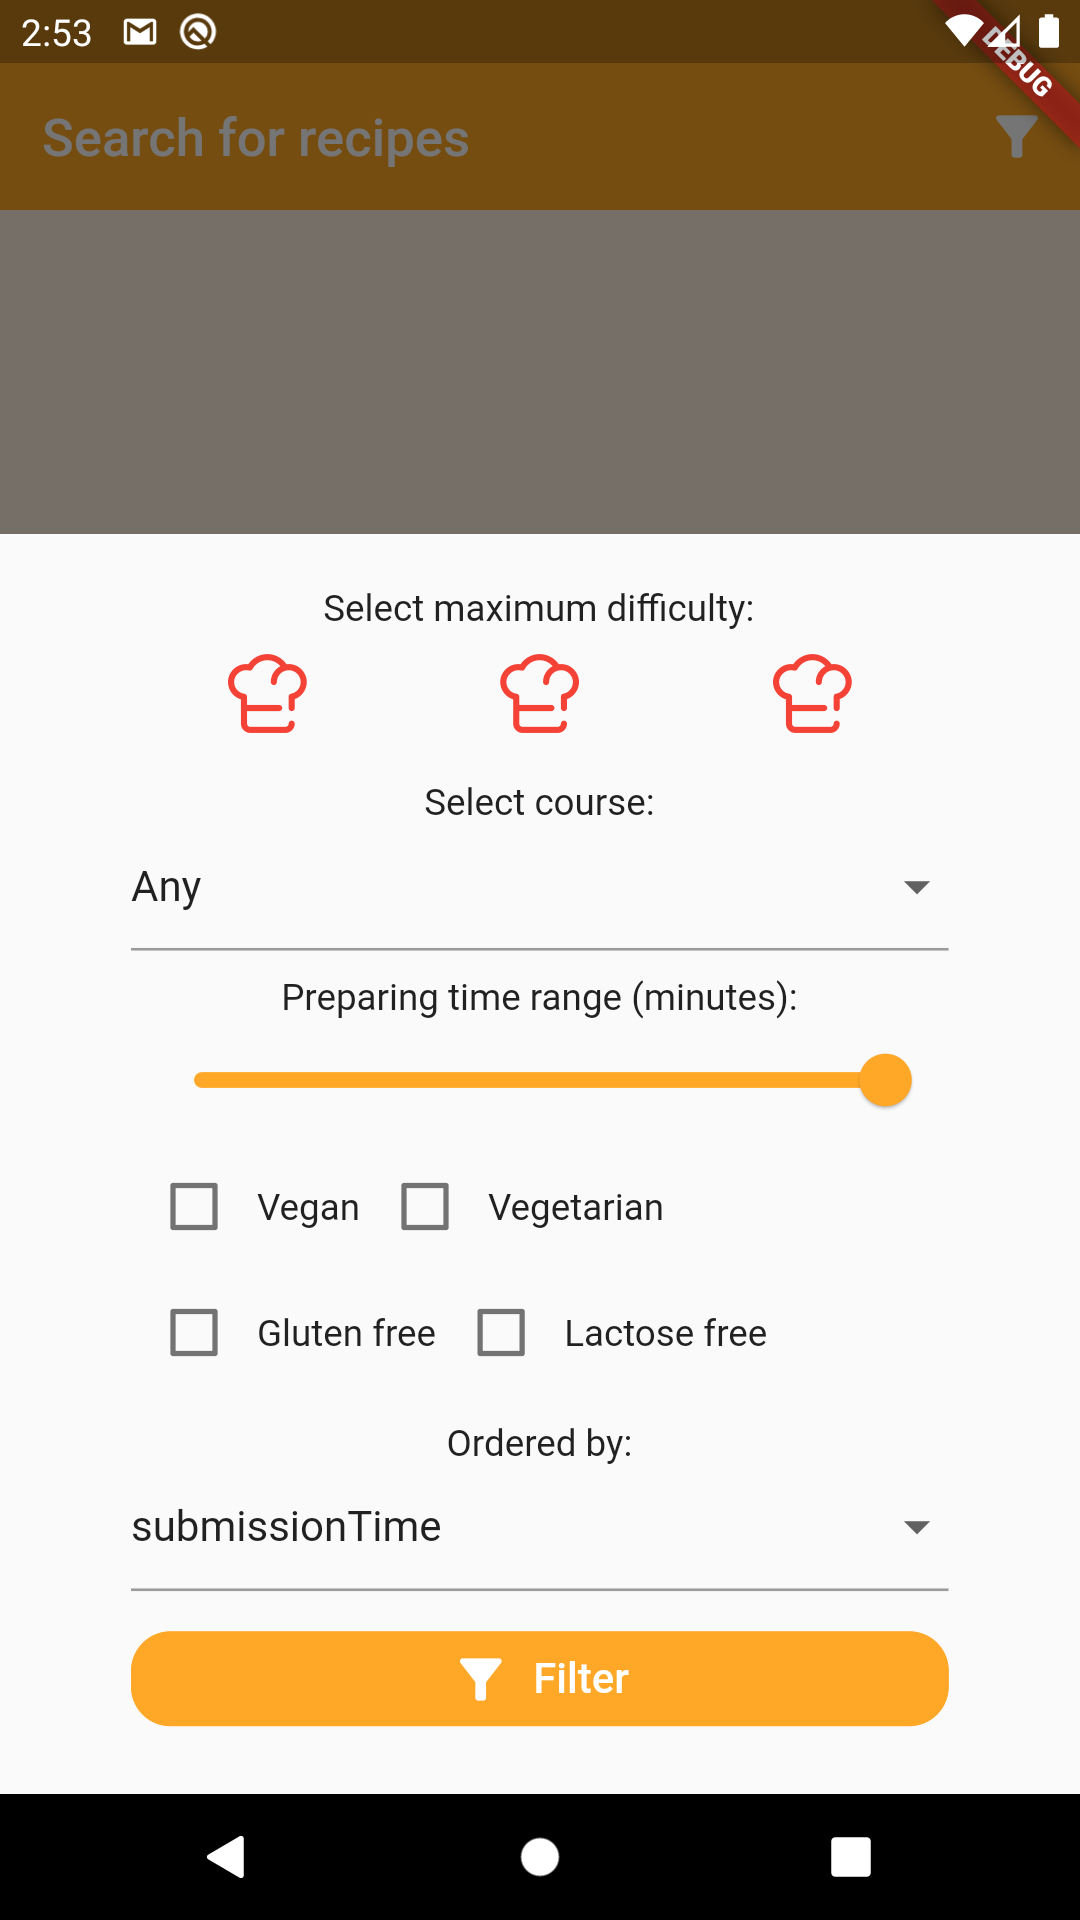
\includegraphics[width = .225\linewidth]{img/Filter.png}
	\caption{Search Recipe Screen}
\end{figure}
This screen, reachable from the home one, gives the possibility to filter the whole database of recipes according to some parameter like duration, difficulty, characteristics...

\subsection{Write and Read Reviews}
\begin{figure}[H]
	\begin{minipage}{0.48\textwidth}
		\centering
		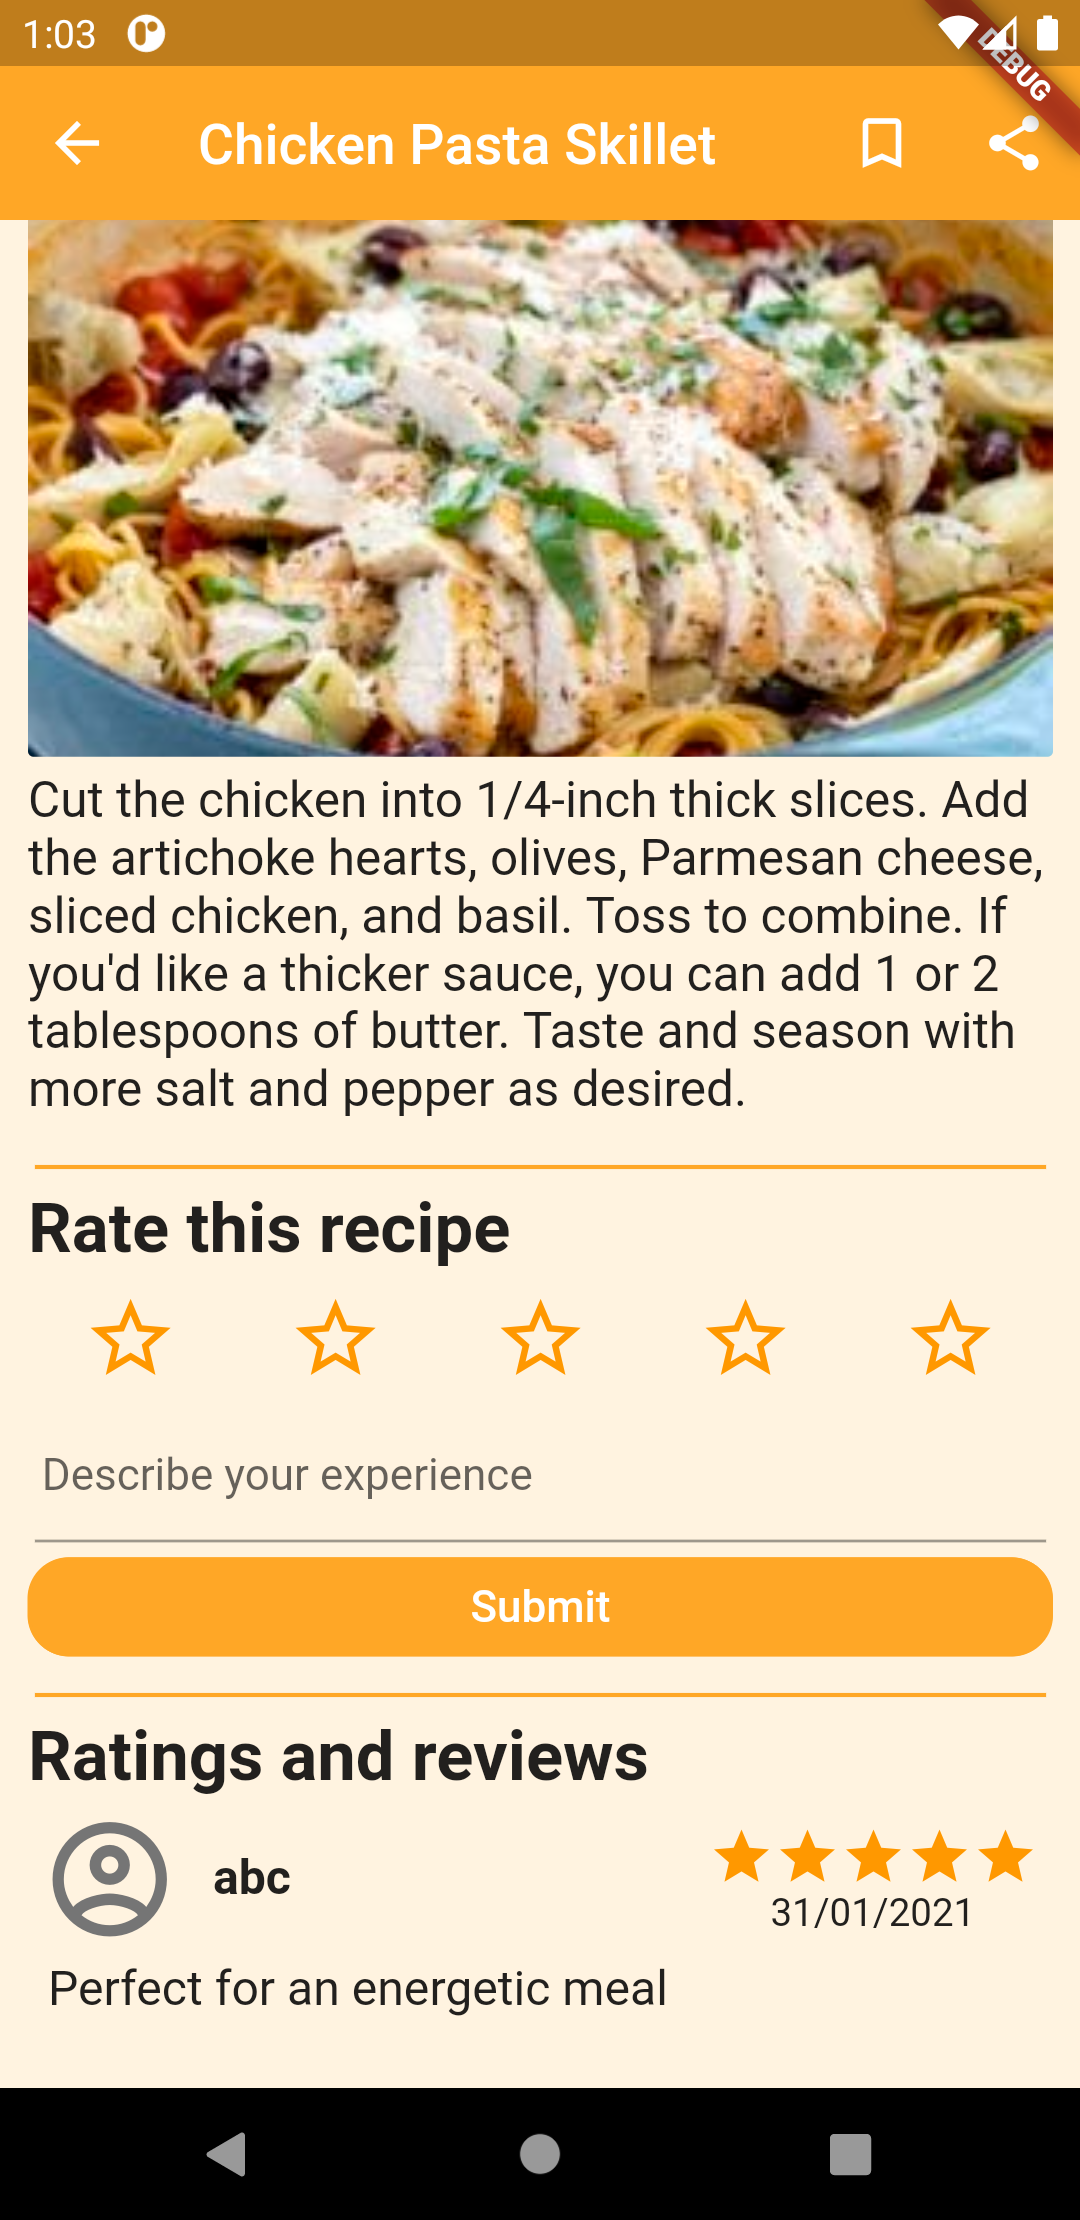
\includegraphics[width = .45\linewidth]{img/Review.png}
		\caption{Write Review Screen}
	\end{minipage}\hfill
	\begin{minipage}{0.48\textwidth}
		\centering
		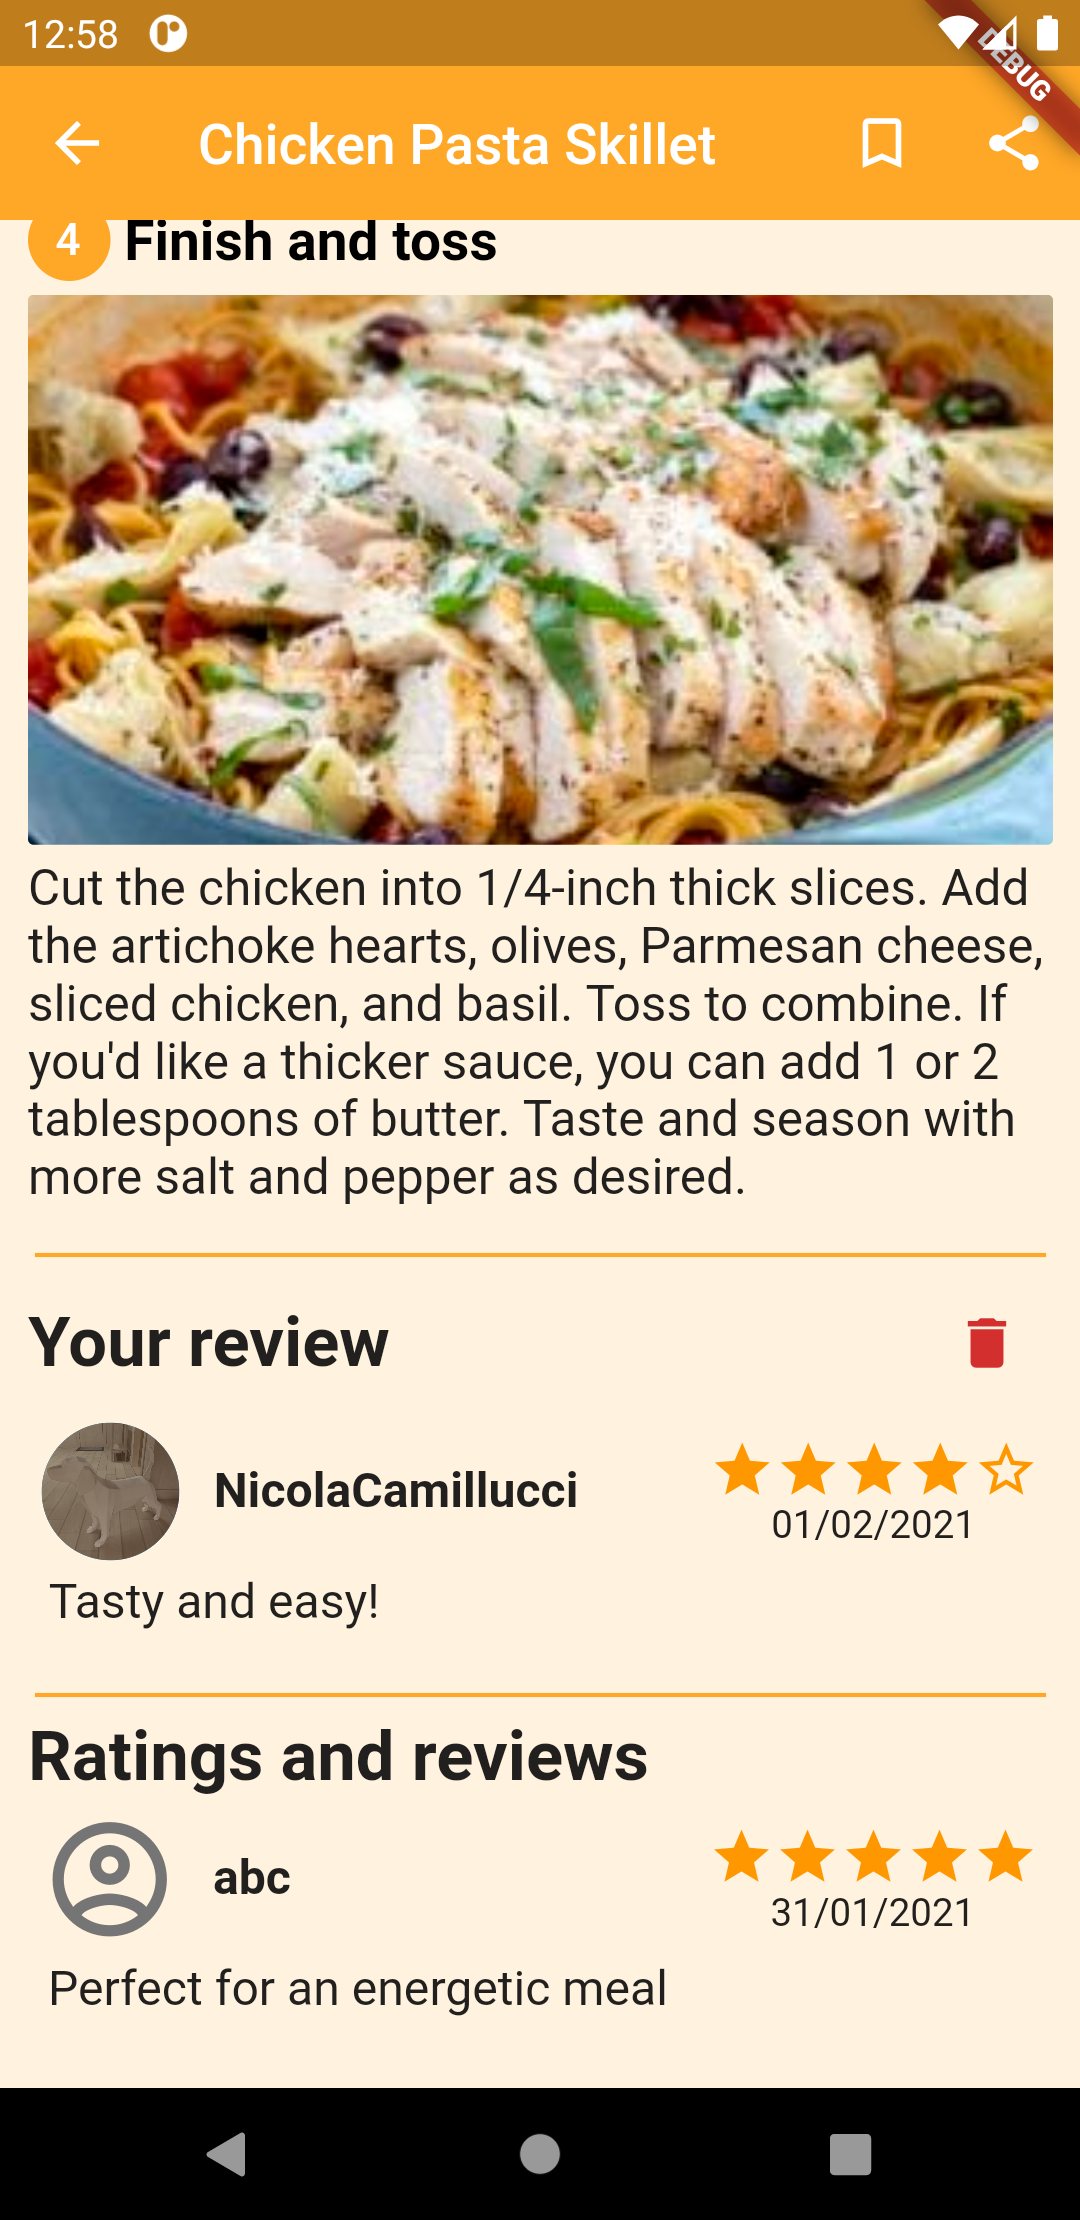
\includegraphics[width = .45\linewidth]{img/Review_2.png}
		\caption{Review View Screen}
	\end{minipage}
\end{figure}

This screen allows the user to leave a review for the visualized recipe, by giving a rating and adding a comment.
Here are also visible the reviews of other users for this recipe, with the authenticated user's review in a separate section.
The review can also be deleted afterwards.

\subsection{Saved Recipes}
\begin{figure}[H]
	\centering
	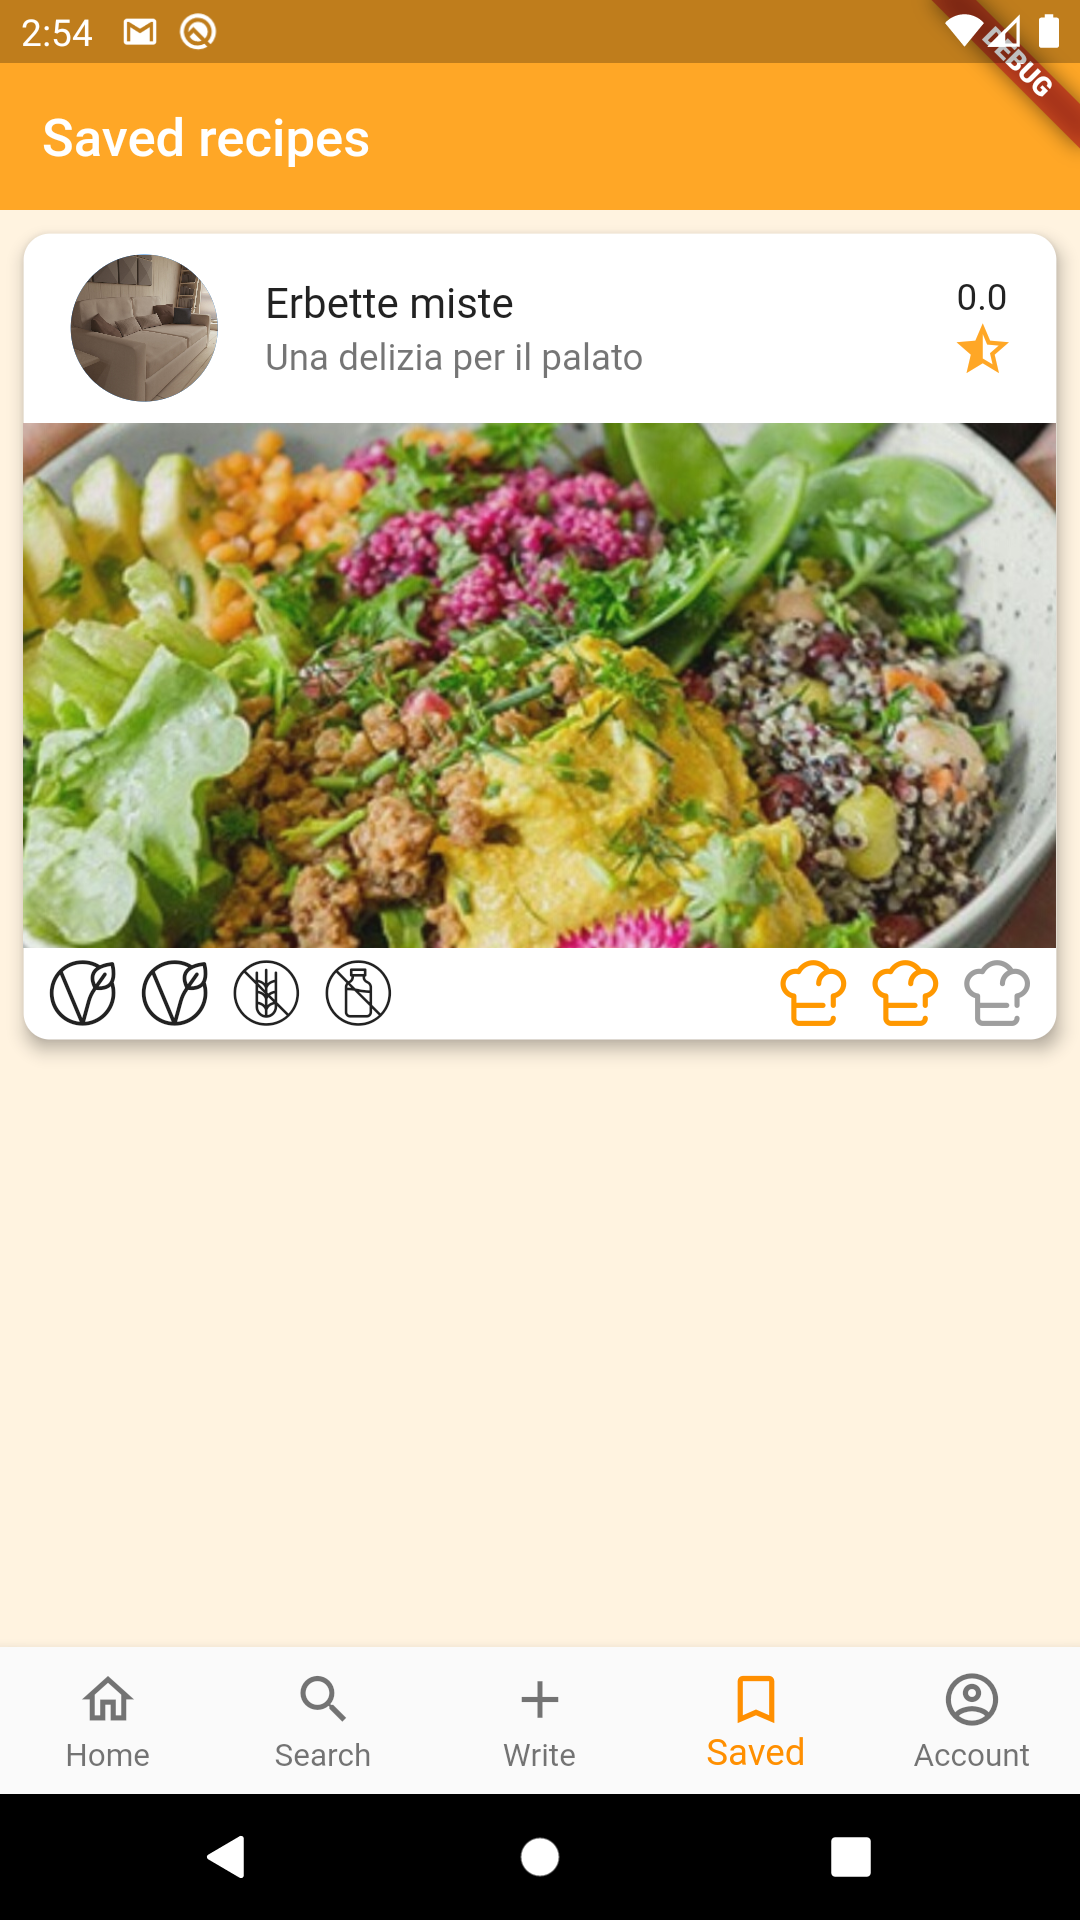
\includegraphics[width = .225\linewidth]{img/Saved.png}
	\caption{Saved Recipe Screen}
\end{figure}
This screen is accessible from the home screen and it lists all the recipes saved by the user displayed in random order.
Recipes can be saved and unsaved by tapping the bookmark icon inside the recipe view.

\subsection{User Profile}
\begin{figure}[H]
	\centering
	\includegraphics[width = .225\linewidth]{img/UserProfile.png}
	\caption{User Profile Screen}
\end{figure}
This screen shows the user profile statistics, which are number of written recipes, number of received reviews and average rating, and the list of the user uploaded recipes.
From here the user can also perform the log out from his/her account.

\subsection{Settings}
\begin{figure}[H]
	\centering
	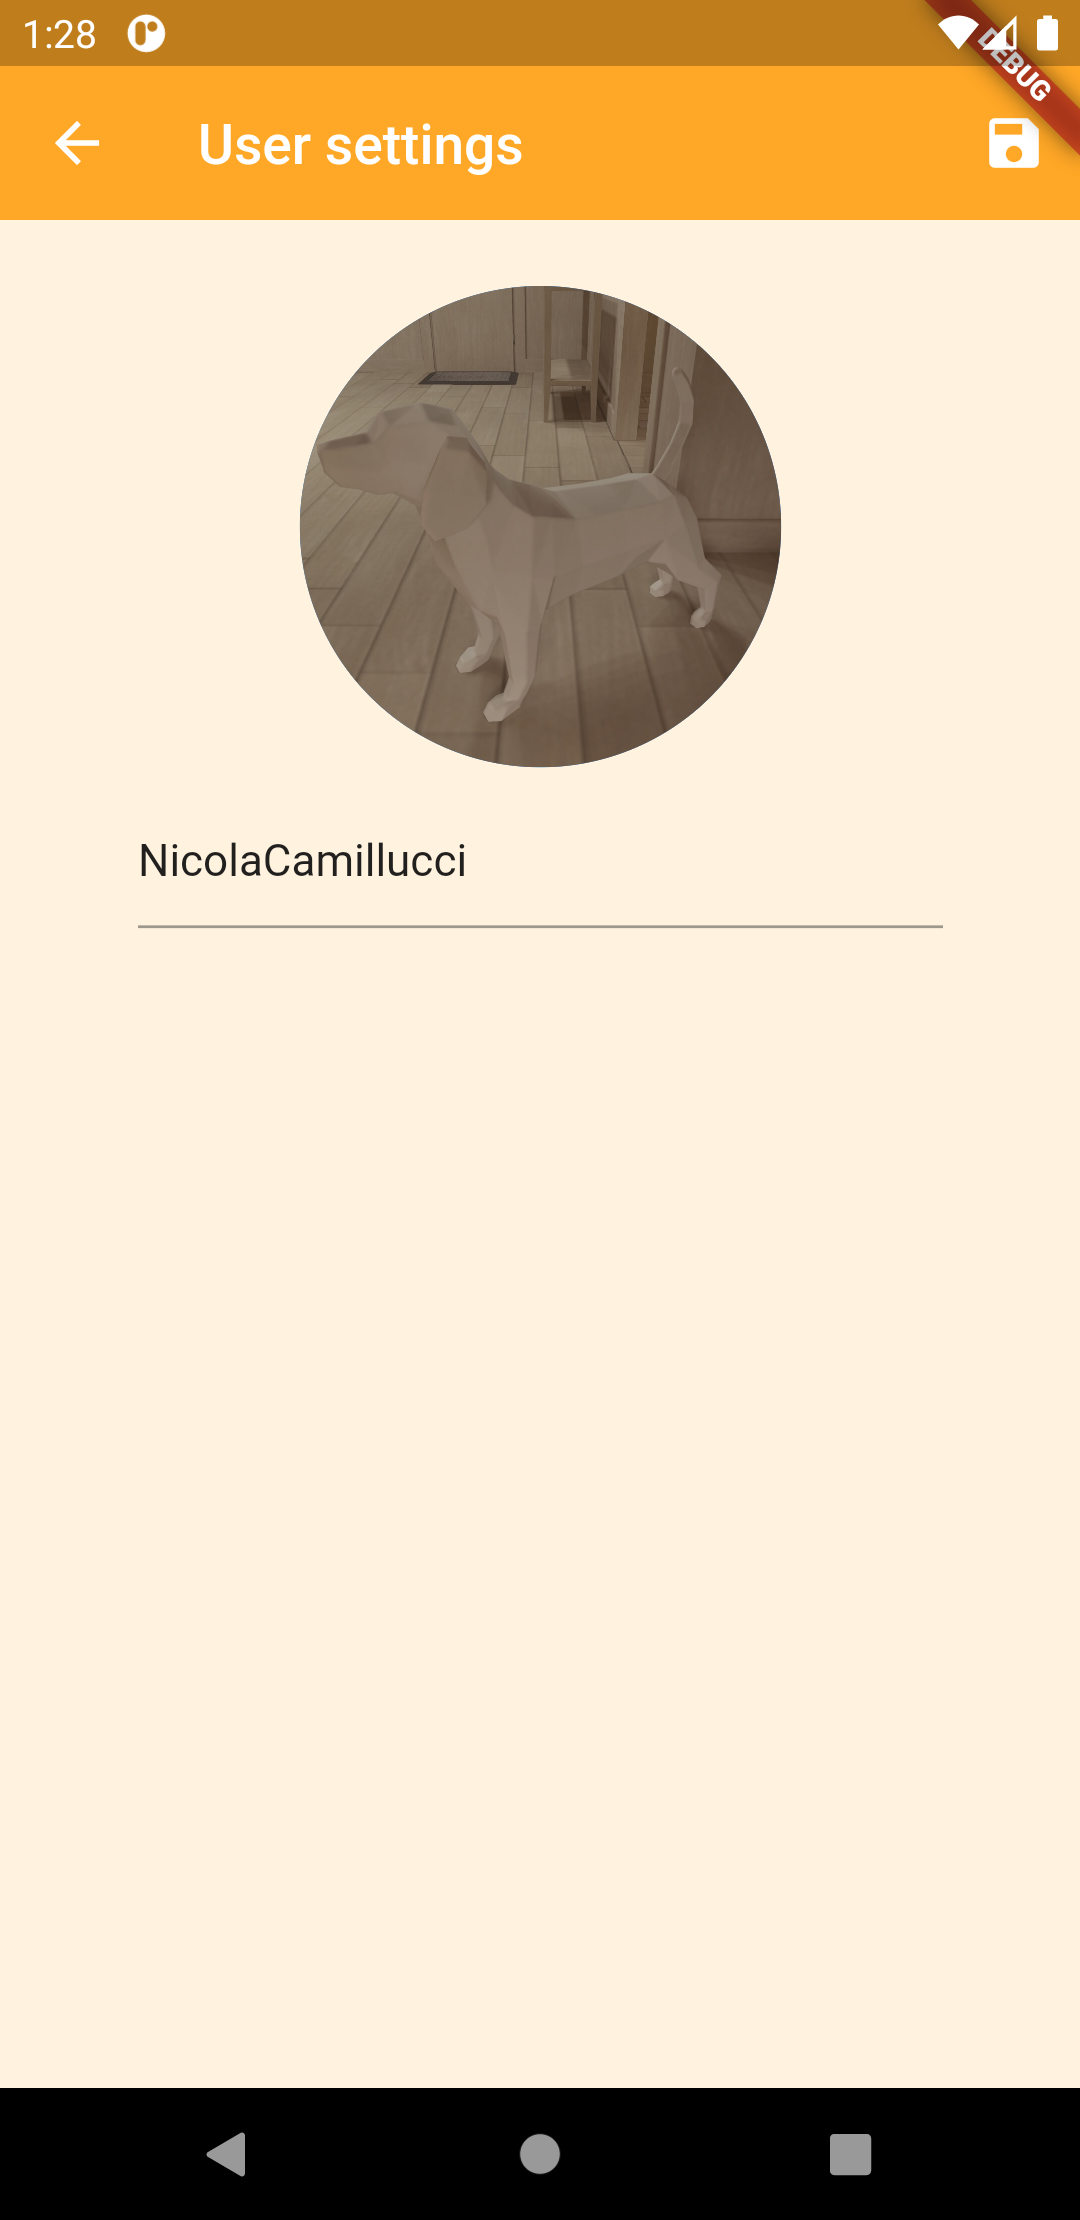
\includegraphics[width = .225\linewidth]{img/Settings.png}
	\caption{Settings Screen}
\end{figure}
This screen allows the user to modify his profile picture, username and the password (only if he is logged using the email).

\newpage
\chapter{Frameworks, External Services and Libraries}

\section{Flutter}
To develop CookingTime application we decided to use Flutter platform, an open source framework, which allows to build cross-platform application basing on Dart programming language. It is developed by Google and allows also the support for web applications.
In order to exploit all the feature of the application as a team we needed to use some other external services that could be easily imported as dependencies into out project environment. 
The usage of all that kind of services helped in terms of reducing the complexity of the implementation and to enforce non-functional requirements like security or authentication tasks.
\begin{figure}[H]
		\begin{center}
			\centering
			
\includegraphics[width=0.35\textwidth]{img/flutterLogo.png}
			\caption{Flutter Logo}
		\end{center}
	\end{figure}
\section{Google Firebase}
Google Firebase is a service offered by Google in order to provide some easily accessible service and to manage critical tasks like authentication in a simpler and smarter way from the perspective of the programmer.
\begin{figure}[H]
		\begin{center}
			\centering
			
\includegraphics[width=0.35\textwidth]{img/firebaseLogo.png}
			\caption{Firebase Logo}
		\end{center}
	\end{figure}
\subsection{Authentication}
The service allowed us to have a unique container for all accounts from the different channel of authentication we offer as email, Facebook and Google account. 
Moreover it is able to manage all the operation without putting in plain text confidential information about user enforced by a SHA-1 encryption. 
The advantage is also the error management as there are specific error codes for each possible evenineces that allowed to provide a better handling of all the possible issues in these critical operations.

\subsection{Cloud Firestore}
Cloud Firestore is part of Firebase, it's basically a database with a document based structure (so NoSQL).
We need it as we have to store data about users and recipes.
Even if the model is NoSQL, we have some instruction provided by the Firebase interface to query the collection of data very similar to SQL one.
We also defined a precise set of rules for the database that restrict unauthorized users to read, create, update or delete documents if they do not have permission to do that action.
Finally, we added some secondary indexes to speed up the query done to the database when needed.

\subsection{Firebase Storage}
As the application has to store picture devoted to profile, dishes and recipe steps, the storage provided by Firestore is the best solution because we are able to access them, after uploading them, through the generated URL within the project online space. 
Of course has there are limitation of the amount of data we can upload, once we modify the pictures we delete the one no more in use.

\section{Social Media}
As mentioned before we implemented the support to authentication using Facebook or Google accounts, this is easily achievable through the API of the platforms.
Basically the APIs convert the credential of the social media account into a token which can be used and stored by Firebase. 
In addition the users are allowed to share a recipe on their preferred social media accounts.

\newpage
\chapter{Test Cases}
The testing phase of CookingTime was split into two steps.

\begin{itemize}
	\item \textbf{Unit test:} In this step we tested some function, like text validators, in order to see if they are behaving in the correct way.
	\item \textbf{Integration-Widget test:} Since all the functionalities of the application are strictly tied with Firebase, we skipped entirely the Widget testing phase and we did a deep integration testing.
	This was the last task performed, in which we automated the testing of the behaviour across multiple widgets and Firebase's services.
\end{itemize}

Here are presented some example of the most relevant test we made:

\section{Unit test}
\begin{table}[H]
	\centering
	\begin{tabular}{|l|l|}
	\hline
	\textbf{Test Case}& Validator Test\\
	\hline
	\textbf{Goal}& input a valid parameter\\
	\hline
	\textbf{Input}& 
	\begin{minipage}{.7\linewidth}
	In one of the application screen,the user insert a valid parameter into a textfield.
	\end{minipage}\\
	\hline
	\textbf{Expected Outcome}& The validator doesn't output any error message.\\
	\hline
	\textbf{Actual Outcome}& 
	\begin{minipage}{.7\linewidth}
	CORRECT: The validator process the input and send it to the requested routine without displaying any error message.
	\end{minipage}\\
	\hline	
	\end{tabular}
	\caption{Validator Test}
\end{table}

\section{Integration-Widget test}
This type of testing was automated for all the feature that are repeatable over the time, while all the non reversible actions were tested manually.

\begin{table}[H]
	\centering
	\begin{tabular}{|l|l|}
	\hline
	\textbf{Test Case}& Successful Login\\
	\hline
	\textbf{Goal}& Login a user\\
	\hline
	\textbf{Input}& 
	\begin{minipage}{.7\linewidth}
	In the login screen the user provides a valid email and password. In the end he taps on login button.
	\end{minipage}\\
	\hline
	\textbf{Expected Outcome}& The user is logged in the and he's routed to the home page.\\
	\hline
	\textbf{Actual Outcome}& 
	\begin{minipage}{.7\linewidth}
	CORRECT: The application allows the user to provide his credential, then tapping the login button the user is logged in the application.
	\end{minipage}\\
	\hline	
	\end{tabular}
	\caption{Successful Login Test}
\end{table}

\begin{table}[H]
	\centering
	\begin{tabular}{|l|l|}
	\hline
	\textbf{Test Case}& Successful Registration\\
	\hline
	\textbf{Goal}& Register a new user\\
	\hline
	\textbf{Input}& 
	\begin{minipage}{.7\linewidth}
	In the login screen the user tap on the registering button, then in the new page provide a valid username, email and password. In the end he taps on register button.
	\end{minipage}\\
	\hline
	\textbf{Expected Outcome}& 
	\begin{minipage}{.7\linewidth}
	The new user is registered and the application routes the user to the home page.
	\end{minipage}\\
	\hline
	\textbf{Actual Outcome}& 
	\begin{minipage}{.7\linewidth}
	CORRECT: The application provides the right screen after clicking on the register button and allows the user to provide his credential, then tapping the registration button the user is registered and logged in the application.
	\end{minipage}\\
	\hline	
	\end{tabular}
	\caption{Successful Registration Test}
\end{table}

\begin{table}[H]
	\centering
	\begin{tabular}{|l|l|}
	\hline
	\textbf{Test Case}& Failed Registration\\
	\hline
	\textbf{Goal}& Try to register a new user omitting some required information\\
	\hline
	\textbf{Input}& 
	\begin{minipage}{.7\linewidth}
	In the login screen the user taps on the registration button, then in the new page provides one or two among valid username, email and password. In the end he taps on register button.
	\end{minipage}\\
	\hline
	\textbf{Expected Outcome}&
	\begin{minipage}{.7\linewidth}
	The new user is not registered and the application throws some alert on the screen.
	\end{minipage}\\
	\hline
	\textbf{Actual Outcome}& 
	\begin{minipage}{.7\linewidth}
	CORRECT: The application provides the right screen after clicking on the register button and allows the user to provide his credential, then tapping the registration button the user is not registered and alerts are thrown.
	\end{minipage}\\
	\hline	
	\end{tabular}
	\caption{Failed Registration Test}
\end{table}

\begin{table}[H]
	\centering
	\begin{tabular}{|l|l|}
	\hline
	\textbf{Test Case}& Successful Password Reset\\
	\hline
	\textbf{Goal}& Reset the password of a user who lost it\\
	\hline
	\textbf{Input}& 
	\begin{minipage}{.7\linewidth}
	In the login screen the user tap on the forgot password button, then in the new page provide email of the account. In the end he taps on send reset email button.
	\end{minipage}\\
	\hline
	\textbf{Expected Outcome}& The user gets a mail to reset his password.\\
	\hline
	\textbf{Actual Outcome}& 
	\begin{minipage}{.7\linewidth}
	CORRECT: The application provides the right screen after clicking on the forgot password button and allows the user to provide his email, then tapping the send reset email button the user receives the reset email.
	\end{minipage}\\
	\hline	
	\end{tabular}
	\caption{Successful Password Reset Test}
\end{table}

\begin{table}[H]
	\centering
	\begin{tabular}{|l|l|}
	\hline
	\textbf{Test Case}& Failed Password Reset\\
	\hline
	\textbf{Goal}& Try to reset the password of a user who lost it omitting the email\\
	\hline
	\textbf{Input}& 
	\begin{minipage}{.7\linewidth}
	In the login screen the user taps on the forgot password button, then he taps on send reset email button without providing the email.
	\end{minipage}\\
	\hline
	\textbf{Expected Outcome}& The user doesn't get a mail to reset his password.\\
	\hline
	\textbf{Actual Outcome}& 
	\begin{minipage}{.7\linewidth}
	CORRECT: The application provides the right screen after clicking on the forgot password button and then tapping the send reset email button the user doesn't receive the reset email.
	\end{minipage}\\
	\hline	
	\end{tabular}
	\caption{Failed Password Reset Test}
\end{table}

\begin{table}[H]
	\centering
	\begin{tabular}{|l|l|}
		\hline
		\textbf{Test Case}& Correct Visualization of a Recipe\\
		\hline
		\textbf{Goal}& Check the correct loading and visualization of a recipe\\
		\hline
		\textbf{Input}& 
		\begin{minipage}{.7\linewidth}
			In the homepage screen the user taps on the first recipe card available and scroll down to the bottom.
		\end{minipage}\\
		\hline
		\textbf{Expected Outcome}& All the elements of the recipe are correctly loaded and visualized.\\
		\hline
		\textbf{Actual Outcome}& 
		\begin{minipage}{.7\linewidth}
			CORRECT: The application provides the right screen after clicking on the recipe card button and then while scrolling through the bottom all widget that display the recipe attributes are displayed.
		\end{minipage}\\
		\hline	
	\end{tabular}
	\caption{Correct Visualization of a Recipe Test}
\end{table}

\begin{table}[H]
	\centering
	\begin{tabular}{|l|l|}
		\hline
		\textbf{Test Case}& Successful Writing Updating and Deleting of a Recipe\\
		\hline
		\textbf{Goal}&Create, visualize, update and delete a recipe\\
		\hline
		\textbf{Input}& 
		\begin{minipage}{.7\linewidth}
			The user goes in the write a recipe screen by tapping the write button on the bottom menu, insert all the information necessary and submit the recipe. Than he verify the presence of the recipe in the user's profile, from there he first modify it and then delete it.
		\end{minipage}\\
		\hline
		\textbf{Expected Outcome}& The user can create, visualize, update and delete a recipe.\\
		\hline
		\textbf{Actual Outcome}& 
		\begin{minipage}{.7\linewidth}
			CORRECT: The application allows the user to submit the recipe only when all the required data is inputted. Then the user can correctly visualize his recipe in both the homepage and user profile page, from which he can access it, modify it and delete it. After the deletion the recipe is correctly not visible anymore.
		\end{minipage}\\
		\hline	
	\end{tabular}
	\caption{Successful Writing Updating and Deleting of a Recipe Test}
\end{table}

\begin{table}[H]
	\centering
	\begin{tabular}{|l|l|}
		\hline
		\textbf{Test Case}& Successful Writing and Deleting of a Review\\
		\hline
		\textbf{Goal}& Crete, visualize and delete a review\\
		\hline
		\textbf{Input}& 
		\begin{minipage}{.7\linewidth}
			From the home screen the user checks the first recipe available and scroll up to to the review form. He then write a review with rating and comment and submit it. After the review is correctly visualized the user deletes the review.
		\end{minipage}\\
		\hline
		\textbf{Expected Outcome}& The user can properly create, visualize and delete their review.\\
		\hline
		\textbf{Actual Outcome}& 
		\begin{minipage}{.7\linewidth}
			CORRECT: The application allows the user to reach and write a review under a recipe. Then the user can correctly visualize his review and can correctly delete his review after a confirmation prompt. The review is then correctly no long available.
		\end{minipage}\\
		\hline	
	\end{tabular}
	\caption{Successful Writing and Deleting of a Review Test}
\end{table}

\begin{table}[H]
	\centering
	\begin{tabular}{|l|l|}
	\hline
	\textbf{Test Case}& Filter Recipes\\
	\hline
	\textbf{Goal}& 
	\begin{minipage}{.7\linewidth}
	The user goes in the search screen and select some parameter to filter the recipes and the ones listed out are retrieved according to the specified parameters.
	\end{minipage}\\
	\hline
	\textbf{Input}& 
	\begin{minipage}{.7\linewidth}
	In the home screen the user taps on the search button on the bottom menu, then he taps the filter button and select some parameters.
	\end{minipage}\\
	\hline
	\textbf{Expected Outcome}& 
	\begin{minipage}{.7\linewidth}
	The application shows only recipes according the parameters selected by the user.
	\end{minipage}\\
	\hline
	\textbf{Actual Outcome}& 
	\begin{minipage}{.7\linewidth}
	CORRECT: The application provides the right screen after clicking on the search button and tapping the filter the user in able to select some parameters in order to filter the recipes, after filtering the retrieved recipes are queried according to the parameter specified before.
	\end{minipage}\\
	\hline	
	\end{tabular}
	\caption{Filter Recipes Test}
\end{table}

\begin{table}[H]
	\centering
	\begin{tabular}{|l|l|}
		\hline
		\textbf{Test Case}& Show User Saved Recipes\\
		\hline
		\textbf{Goal}& See saved recipes in the saved recipe view\\
		\hline
		\textbf{Input}& 
		\begin{minipage}{.7\linewidth}
			From the homepage screen the user checks that the saved recipes view is empty. Then from the latest recipes view he saves the first two recipes and checks them in the saved recipes view, where they should be present. He then un-saves one of the two and controls that only the remaining one is still visible. He finally un-saves the other recipe and checks that there no saved recipes anymore.
		\end{minipage}\\
		\hline
		\textbf{Expected Outcome}&
		\begin{minipage}{.7\linewidth}
		The user can properly add, visualize and remove recipes form the saved recipes view.
		\end{minipage}\\
		\hline
		\textbf{Actual Outcome}& 
		\begin{minipage}{.7\linewidth}
			CORRECT: The application allows the user to save and visualize saved recipes in the correct widget on the homepage. He can then add further recipes and remove old one, after which they are no longer visualized.
		\end{minipage}\\
		\hline	
	\end{tabular}
	\caption{Show User Saved Recipes Test}
\end{table}

\begin{table}[H]
	\centering
	\begin{tabular}{|l|l|}
	\hline
	\textbf{Test Case}& Show User information and recipes\\
	\hline
	\textbf{Goal}& See correct user data and recipes\\
	\hline
	\textbf{Input}& 
	\begin{minipage}{.7\linewidth}
	In the home screen the user taps the account button in the bottom menu.
	\end{minipage}\\
	\hline
	\textbf{Expected Outcome}& 
	\begin{minipage}{.7\linewidth}
	The user is able to see his personal information, his statistics and his recipes.
	\end{minipage}\\
	\hline
	\textbf{Actual Outcome}&
	\begin{minipage}{.7\linewidth}
	CORRECT: The application allows the user to see the profile picture, username, written recipes and received reviews after tapping the account button in the home page.
	\end{minipage}\\
	\hline	
	\end{tabular}
	\caption{Show User information and recipes}
\end{table}

\begin{table}[H]
	\centering
	\begin{tabular}{|l|l|}
	\hline
	\textbf{Test Case}& Change user information\\
	\hline
	\textbf{Goal}& Modify profile picture, username and password\\
	\hline
	\textbf{Input}& 
	\begin{minipage}{.7\linewidth}
	In the home screen the user taps the account button in the bottom menu, then he goes in the setting page through the setting button and inserts new information and presses the save button.
	\end{minipage}\\
	\hline
	\textbf{Expected Outcome}& The user is able to see his updated personal information.\\
	\hline
	\textbf{Actual Outcome}& 
	\begin{minipage}{.7\linewidth}
	CORRECT: The application allows the user to set a new profile picture, username and password. After tapping the save button he is able to see the modified information updated.
	\end{minipage}\\
	\hline	
	\end{tabular}
	\caption{Change user information}
\end{table}
\newpage
\chapter{Cost Estimation}
In this section we include a cost estimation for CookingTime application development. In order to exploit the estiaton we decided to use COCOMO (Constructive Cost Model) model. The usage of this analysis tool allow us to determine the time required for the developemnt of this type of appliaction.
First of all we have to decide what type of project we are producing in order to take the right estimation parameters, according to the following table.
%TODO table of coefficient
The classes of COCOMO represent different difficulties of the product and experiences of developers, espelly:
\begin{itemize}}
	\item \textbf{Organic} It means small project done by small teams with a good experience and low constraints.
	\item \textbf{Semi-Detached} It means project with a significant large team with different experiences and medium constraints.
	\item \textbf{Embedded} It means we have tight constraints and a mixture of Organic and Semi-Detached classes of projects.
\end{itemize}
Then we can consider the equation to represent the effort spent:
%effort = a*(KLOC)^b
$ effort = a * (KOLOC)^{b}$
%duration = c*effort^d
$ duration = c * effort^{d}$
where \textbf{KLOC} are the estiamted number of thousand lines of code, \textbf{effort} expressed in man-months and the duration is the time estimeted to be taken in order to develop the application.

Even if it was the first time we developed a mobile application, we have good bases in coding moreover the project is simple and without tight constraints, so we can consider our project as organic, also because we have a team composed by two students.

%TODO outcome of formulas

%TODO outcome related to each of us  
\newpage
\chapter{Future Works}
In this section we will present future possible improvements for CookingTime application.
\begin{itemize}
	\item Give some badges in order to make fidelization of user and to give prizes to most active and productive user.
	\item Notification system, to let the user know when another user reviewed his/her recipes. 
	\item Possibility to add ingredients required for a recipe to a shopping list. This allows people to take what they need to prepare some of the recipes.
	\item Add additional categories to group more finely different types of recipes.
	\item Allow users to search recipes by title or by ingredient, specifying a text to search for.
	\item Allow users to check other users profile, in order to see their statistics and other recipes they wrote.
\end{itemize}
These are the main improvements we can implement after the release of the application, but as everyone know, this type of app, which allows user to interact and share something from their own lives, has no limit of improvement about features, user experience and layout.


\end{document} 
